\documentclass[italian]{unicam-thesis}

\title{Compilazione di un linguaggio funzionale in Java}

\university{Università degli Studi di Camerino}
\school{Scienze e Tecnologie}
\course{Laurea in Informatica (Classe L-31)}

\author{Massimo Pavoni}
\advisor{Prof. Luca Padovani}
\academicyear{2023/2024}
\matricola{124377}

\graphicspath{{resources/images/}}

\addbibresource{8-bibliography.bib}

\begin{document}

\pagenumbering{roman}

\maketitle

\tableofcontents

\begingroup
\let\cleardoublepage\relax
\let\clearpage\relax

\lstlistoflistings

\listoffigures

\listoftables

\endgroup

\cleardoublepage

\pagenumbering{arabic}

\chapter{\localized{Introduzione}{Introduction}}
\label{chap:1-introduction}

Lorem ipsum dolor sit amet, \index{consectetur} adipisci elit, sed do eiusmod tempor incidunt ut labore et dolore magna aliqua. Ut enim ad minim veniam, quis nostrum exercitationem ullamco laboriosam, nisi ut aliquid ex ea commodi consequatur. Duis aute irure reprehenderit in voluptate velit esse cillum dolore eu fugiat nulla pariatur. Excepteur sint obcaecat cupiditat non proident, sunt in culpa qui officia deserunt mollit anim id est laborum.

Nel Capitolo \ref{chap:1-introduction} illustreremo prima le motivazioni che ci hanno spinto a perseguire l'obiettivo descritto e quindi la struttura della tesi.

\section{Motivazione}
\section{Obiettivi}
\section{Struttura della Tesi}

\chapter{Funx}
\label{chap:2-funx}

Questo capitolo descrive brevemente i linguaggi funzionali e le scelte effettuate
durante l'ideazione del linguaggio usato per il progetto: \textbf{Funx}.

\noindent Il nome nasce dall'unione dei due termini anglosassoni \textit{functional} e \textit{expression};
viene quindi pronunciato \textipa{["f2nIk"s]} in inglese,
\textipa{[fan\textperiodcentered èks]} o \textipa{[fan\textperiodcentered ìks]} in italiano.

\section{Linguaggi funzionali}
\label{sec:2-1-functional-languages}

Nonostante i linguaggi di programmazione non si possano confinare all'interno di un solo paradigma,
parlando di linguaggi di programmazione si fa comunque spesso riferimento a due grandi categorie:
linguaggi imperativi e linguaggi dichiarativi.


I primi hanno caratteristiche direttamente legate al modello di calcolo di \textit{John Von Neumann},
a sua volta non dissimile dalla macchina di \textit{Alan Turing}.
Questi linguaggi sono usati per codice che segue una precisa sequenza di istruzioni,
la quale descrive più o meno esplicitamente i passi necessari per risolvere il problema affrontato.

\noindent Appartengono alla famiglia dei linguaggi di programmazione imperativi sia linguaggi procedurali come
\texttt{Fortran}, \texttt{Cobol} e \texttt{Zig}, sia i linguaggi orientati agli oggetti, tra cui \texttt{Kotlin}, \texttt{C\#} e \texttt{Ruby}.


I linguaggi dichiarativi, invece, sono fondamentali per lo scopo del progetto:
tali linguaggi sono generalmente di altissimo livello e permettono allo sviluppatore
di concentrarsi sull'obiettivo da raggiungere piuttosto che sui dettagli implementativi.

\noindent Fanno parte di questa categoria linguaggi di interrogazione come \texttt{SQL},
linguaggi logici come \texttt{Prolog} e soprattutto i linguaggi funzionali:
\texttt{Lisp}, \texttt{Clojure}, \texttt{Elixir}, \texttt{OCaml} e \texttt{Haskell} sono alcuni esempi.


Alla base dei linguaggi funzionali vi è il \textbf{lambda calcolo} {\cite{Church-1932-FoundationLogic,Church-1933-FoundationLogic}}:
un sistema formale definito dal matematico \textit{Alonzo Church} (supervisore di \textit{Alan Turing} durante il dottorato),
equivalente alla macchina di Turing, ma fondato sulle funzioni pure.

\newpage

\noindent La grammatica del lambda calcolo verrà presentata poco più avanti (sezione~\ref{sec:2-3-syntax}),
ma le regole che ne governano il funzionamento e il modo in cui queste vengano utilizzate per ridurre
le espressioni ad una forma normale esulano dai fini di questo documento.

\noindent Rimane comunque rilevante elencare le principali qualità che un linguaggio funzionale
usualmente matura grazie al lambda calcolo:
\begin{itemize}
      \item \textbf{funzioni come entità di prima classe}: le funzioni possono essere passate come argomenti
            e restituite come risultato di altre funzioni;
      \item \textbf{immutabilità}: le variabili utilizzate sono immutabili;
      \item \textbf{purezza}: le funzioni sono libere da effetti collaterali
            (non modificano lo stato del programma) e restituiscono sempre lo stesso output per input identici;
      \item \textbf{ricorsione}: la ricorsione è il meccanismo più idiomatico per esprimere
            l'iterazione su una struttura dati.
\end{itemize}

\subsection{ML, Haskell e Funx}
\label{sec:2-2-ml-haskell-funx}

Nonostante le funzioni pure tipiche di un linguaggio funzionale siano un concetto molto attraente
dal punto di vista della correttezza della computazione, i vincoli così imposti possono risultare
stringenti a tal punto da rendere difficile, se non impossibile, la scrittura di programmi che
interagiscano con il mondo reale.


Per questo motivo, molti linguaggi funzionali permettono invece di utilizzare particolari funzioni
impure o di effettuare almeno operazioni di input/output. Inoltre, molti linguaggi prevalentemente
imperativi adottano ormai da tempo alcune caratteristiche tipiche dei linguaggi funzionali
(e.g. \texttt{Rust}, il linguaggio più amato%
\footnote{Stack Overflow Developer Survey 2023 (\url{https://survey.stackoverflow.co/2023}), \\
    \textit{Rust is the most admired language}}
dagli sviluppatori secondo i sondaggi di \textit{Stack Overflow},
eredita molto dal linguaggio con cui era scritto il suo primo compilatore, \texttt{OCaml}, ed è dotato quindi di
funzioni di prima classe, immutabilità di default, strutture dati algebriche, ecc.).


\texttt{ML} è un linguaggio funzionale sviluppato negli anni '70 presso l'Università di Edimburgo,
costituente la base per moltissimi dei linguaggi sviluppati in seguito.
\texttt{ML} permette effettivamente l'uso di funzioni impure, ma fra i suoi discendenti
vi è \texttt{Haskell}, uno dei pochi linguaggi invece completamente puri.

\noindent \texttt{Haskell} si avvale di un pattern di programmazione chiamato \textit{monadi} {\cite{Moggi-1991-ComputationMonads}}
per gestire le operazioni di input/output e altre impurità, mantenendo le funzioni pure.


Nell'ideare \textbf{Funx} l'ispirazione viene proprio da \texttt{Haskell}, ma è presente la possibilità
di dichiarare un'unica funzione impura (il cosiddetto \textit{main}) per permettere di visualizzare a schermo un risultato.
Il linguaggio non è quindi allo stesso livello di purezza di \texttt{Haskell}, e naturalmente non supporta
molte delle funzionalità più avanzate di quest'ultimo (come le \textit{classi di tipi} e il \textit{pattern matching}),
ma ne mutua altre comunque interessanti, tra cui l'uso di alcuni operatori infissi e il \textit{polimorfismo parametrico}.

\newpage

\section{Sintassi}
\label{sec:2-3-syntax}

La sintassi di \textbf{Funx} risulta molto simile a quella di \texttt{Haskell}, con poche differenze dovute
a tre principali motivi:
\begin{itemize}
    \item libera scelta di nomi e simboli per le parole chiave;
    \item necessità di successiva traduzione in \texttt{Java};
    \item difficoltà e scarso valore all'interno del progetto dell'implementazione di un parser dipendente dall'indentazione.
\end{itemize}

\noindent A prescindere da ciò, il cuore del linguaggio è lo stesso di ogni altro linguaggio derivato dal lambda calcolo:
la sua definizione si può agilmente comprendere visualizzando la grammatica del lambda calcolo e confrontandola con
quella (leggermente semplificata) di \textbf{Funx}, facendo attenzione alle regole aggiuntive.

\begin{figure}
    \vspace{4mm}
    \begin{bnf}
        $E$ : \small{Espressione} ::=
        | $x$ : \small{variabile}
        | $E_l\ E_r$ : \small{applicazione}
        | $\lambda x\ .\ E$ : \small{astrazione}
    \end{bnf}
    \caption{Grammatica del lambda calcolo}
    \label{fig:2-3-lambda-syntax}
    \vspace{4mm}
\end{figure}

\noindent Le tre regole in Figura~\ref{fig:2-3-lambda-syntax} indicano le tre componenti indispensabili
del lambda calcolo:
\begin{itemize}
    \item \textbf{variabile}: simbolo rappresentante un parametro;
    \item \textbf{applicazione}: applicazione di funzione ad un argomento (entrambi espressioni);
    \item \textbf{astrazione}: definizione di una funzione anonima, con un solo input $x$ (variabile vincolata)
          e un solo output $E$ (espressione); per definire funzioni con più
          parametri si debbono usare molteplici astrazioni annidate (tecnica detta \textit{currying}).
\end{itemize}

\newpage

\begin{figure}
    \begin{bnf}
        $M$ : \small{Modulo} ::=
        | $nome\ \cdot\ L$
        ;;
        $D$ : \small{Dichiarazione} ::=
        | $?(schema\ di\ tipo)\ \cdot\ id = E$ : \small{funzione}
        ;;
        $E$ : \small{Espressione} ::=
        | $c$ : \small{costante}
        | $x$ : \small{variabile}
        | $E_l\ E_r$ : \small{applicazione}
        | $\lambda x\ .\ E$ : \small{astrazione}
        | $L$ : \small{let}
        | $\textbf{if}\ E_c\ \textbf{then}\ E_t\ \textbf{else}\ E_e$ : \small{if}
        ;;
        $L$ : \small{Let} ::=
        | $\textbf{let}\ \cdot\ D\ (\cdot\ D)^*\ \cdot\ \textbf{in}\ E$
    \end{bnf}
    \caption{Grammatica di \textbf{Funx}}
    \label{fig:2-3-funx-syntax}
    \vspace{4mm}
\end{figure}

\noindent È facile constatare la presenza delle ulteriori produzioni per la definizione del modulo corrente
(informazione inclusa a prescindere dal fatto che il linguaggio ad ora non supporti l'importazione di moduli esterni
che non siano la libreria standard) e di funzioni con nome: lo \textit{schema di tipo} è un'informazione opzionale
relativa al tipo della funzione e di cui si parlerà più approfonditamente nella sezione~\ref{sec:3-3-system-fc}.

\noindent Per quanto riguarda invece le espressioni, vengono introdotte tre nuove regole:
\begin{itemize}
    \item \textbf{costante}: rappresenta un valore letterale, come un numero o una stringa;
    \item \textbf{let}: permette di avere dichiarazioni locali utilizzabili all'interno di un'espressione;
    \item \textbf{if}: la più classica istruzione condizionale controllata da un'espressione booleana.
\end{itemize}

\subsection{Zucchero sintattico}
\label{sec:2-4-syntactic-sugar}

Con lo scopo di rendere il codice più leggibile, conciso e semplice, \textbf{Funx} introduce
dello zucchero sintattico (del tutto simile a quello di \texttt{Haskell}).
In Tabella~\ref{tab:2-4-sugar} sono riportati l'indispensabile per evitare il parsing dell'indentazione,
le semplificazioni comuni utili all'arricchimento del lambda calcolo, e infine tutti gli operatori simbolici
supportati al momento (assieme alla notazione per indicarne associatività e precedenza).

\newpage

\begin{table}[H]
    \begin{center}
        \begin{tabularx}{\textwidth}{|P{15em}|X|}
            \hline
            \textbf{Zucchero}                & \textbf{Sostituzione}                                            \\
            \hline
            \texttt{$\backslash$x -> e}      & \texttt{$\lambda$x $\mathord{.}$ e}                              \\
            \hline
            \texttt{$\backslash$x y -> e}    & \texttt{$\lambda$x $\mathord{.}$ $\lambda$y $\mathord{.}$ e}     \\
            \hline
            \texttt{f x y = e}               & \texttt{f = $\lambda$x $\mathord{.}$ $\lambda$y $\mathord{.}$ e} \\
            \hline
            \texttt{let}                     &                                                                  \\
            \texttt{f1 = e1}                 & \texttt{let f1 = e1 $\cdot$ f2 = e2 in e3}                       \\
            \texttt{f2 = e2}                 &                                                                  \\
            \texttt{in e3}                   &                                                                  \\
            \hline
            \texttt{f3 = e3}                 &                                                                  \\
            \texttt{with}                    &                                                                  \\
            \texttt{f1 = e1}                 & \texttt{f3 = let f1 = e1 $\cdot$ f2 = e2 in e3}                  \\
            \texttt{f2 = e2}                 &                                                                  \\
            \texttt{out}                     &                                                                  \\
            \hline
            \texttt{main = e3}               &                                                                  \\
            \texttt{f1 = e1}                 & \texttt{main = let f1 = e1 $\cdot$ f2 = e2 in e3}                \\
            \texttt{f2 = e2}                 &                                                                  \\
            \hline
            \texttt{if b then e1 else e2 fi} & \texttt{if b then e1 else e2}                                    \\
            \hline
        \end{tabularx}
        % divide et impera because inconsistent tabbing is a thing
        \begin{tabularx}{\textwidth}{|P{7em}@{\quad}P{7em}|X|}
            \texttt{e1 $\mathord{.}$ e2} & \texttt{infixr 9} & \texttt{compose e1 e2}            \\
            \texttt{e1 / e2}             & \texttt{infixl 7} & \texttt{divide e1 e2}             \\
            \texttt{e1 \% e2}            & \texttt{infixl 7} & \texttt{modulo e1 e2}             \\
            \texttt{e1 * e2}             & \texttt{infixl 7} & \texttt{multiply e1 e2}           \\
            \texttt{e1 + e2}             & \texttt{infixl 6} & \texttt{add e1 e2}                \\
            \texttt{e1 - e2}             & \texttt{infixl 6} & \texttt{subtract e1 e2}           \\
            \texttt{e1 > e2}             & \texttt{infix 4}  & \texttt{greaterThan e1 e2}        \\
            \texttt{e1 >= e2}            & \texttt{infix 4}  & \texttt{greaterThanEquals e1 e2}  \\
            \texttt{e1 < e2}             & \texttt{infix 4}  & \texttt{lessThan e1 e2}           \\
            \texttt{e1 <= e2}            & \texttt{infix 4}  & \texttt{lessThanEquals e1 e2}     \\
            \texttt{e1 == e2}            & \texttt{infix 4}  & \texttt{equalsEquals e1 e2}       \\
            \texttt{e1 != e2}            & \texttt{infix 4}  & \texttt{notEquals e1 e2}          \\
            \texttt{!!e}                 & \texttt{prefix 4} & \texttt{not e}                    \\
            \texttt{e1 \&\& e2}          & \texttt{infixr 3} & \texttt{if e1 then e2 else False} \\
            \texttt{e1 || e2}            & \texttt{infixr 2} & \texttt{if e1 then True else e2}  \\
            \texttt{e1 \$ e2}            & \texttt{infixr 0} & \texttt{apply e1 e2}              \\
            \hline
        \end{tabularx}
    \end{center}
    \caption{Zucchero sintattico}
    \label{tab:2-4-sugar}
\end{table}

\newpage

\noindent Come già accennato, il Capitolo~\ref{chap:5-compiler} illustrerà come l'albero sintattico astratto (\textbf{AST})
di un programma viene ottenuto, annotato e tradotto in \texttt{Java}; la sezione~\ref{sec:4-2-ternary-operator}
esporrà invece il motivo della traduzione degli operatori booleani binari in if.

\noindent Alcuni esempi di funzioni sono presentati nel Codice~\ref{lst:2-4-example-funx};
seppur superflua, l'indentazione è inclusa per maggiore chiarezza.

\vspace{4mm}
\begin{lstlisting}[caption={Esempio di programma}, style=funxCode, label={lst:2-4-example-funx}]
main = factorial 20

factorial : Int @-> Int
factorial n = if n == 0 then 1 else n * factorial (n - 1) fi

even : Int @-> Bool
even = let
        even1 : Int @-> Bool
        even1 n = if n == 0 then True else odd (n - 1) fi

        odd : Int @-> Bool
        odd n = if n == 0 then False else even1 (n - 1) fi
    in even1

gcd : Int @-> Int @-> Int
gcd a b = if b == 0 then a else gcd b (a % b) fi

xor : Bool @-> Bool @-> Bool
xor a b = (a || b) && !!(a && b)
\end{lstlisting}
\chapter{\localized{Inferenza di tipo}{Type inference}}
\label{chap:3-inference}

Dopo aver discusso la sintassi di \textbf{Funx}, è importante far notare come i programmi
non abbiano bisogno di annotazioni di tipo, nonostante siano stati adottati tipi statici.

\noindent In questo capitolo affronteremo l'argomento dei sistemi di tipo e dell'inferenza,
meccanismo proprio di molti linguaggi, funzionali e non, che rende possibile la deduzione
automatica del tipo di un termine basandosi sull'utilizzo delle variabili e delle funzioni.

\section{Sistemi di tipo}
\label{sec:3-1-type-systems}

Durante la genesi di ogni linguaggio di programmazione, una delle scelte più significative riguarda
l'introduzione di un sistema per gestire i tipi di variabili ed espressioni.

\noindent Tali sistemi di tipo sono di fatto insiemi di regole logiche che permettono
di assegnare una proprietà \textit{"type"} a ciascuno dei termini del linguaggio che ne necessitano.

\noindent Sono principalmente suddivisi in due categorie:
\begin{itemize}
      \item \textbf{tipizzazione statica}: i tipi sono definiti a tempo di compilazione
            e non possono cambiare mentre il programma è in esecuzione;
      \item \textbf{tipizzazione dinamica}: i tipi vengono stabiliti durante l'esecuzione
            e possono cambiare in qualsiasi momento.
\end{itemize}

\noindent Oltre a questa distinzione esistono varie sfumature e approcci differenti,
informalmente classificati in base alla rigidità delle regole di tipizzazione.
Si parla di \textit{tipizzazione debole} quando ad esempio sono consentite conversioni implicite tra tipi diversi,
\textit{tipizzazione forte} se sono impedite, oppure qualora sia o meno disponibile l'aritmetica dei puntatori.

\newpage

\begin{figure}
      \begin{tikzpicture}[scale=0.5, >={Stealth[width=1.5mm,length=2mm]}]
            % nodes instead of proper axis, less of a hassle
            \node (dynamic) at (-11,0) {Dinamico};
            \node (static) at (11,0) {Statico};
            \node (weak) at (0,-11) {Debole};
            \node (strong) at (0,11) {Forte};
            \draw[<->] (dynamic) -- (static);
            \draw[<->] (weak) -- (strong);
            % bleh
            \node at (-8,-5) {\texttt{Visual Basic}};
            \node at (-4,-8) {\texttt{JavaScript}};
            \node at (-8,-2) {\texttt{Perl}};
            \node at (-3,-3) {\texttt{PHP}};
            % meh
            \node at (-7,8) {\texttt{Erlang}};
            \node at (-8,5) {\texttt{Clojure}};
            \node at (-3,7) {\texttt{Groovy}};
            \node at (-6,3) {\texttt{Python}};
            \node at (-2,2) {\texttt{Ruby}};
            % okay
            \node at (3,-4) {\texttt{C}};
            \node at (6,-6) {\texttt{C++}};
            % good
            \node at (3,7) {\texttt{C\#}};
            \node at (4,1) {\texttt{Funx}}; % bleh amongst the good
            \node at (5,4) {\texttt{Java}};
            \node at (2,3) {\texttt{F\#}};
            \node at (7,6) {\texttt{Scala}};
            \node at (8,2) {\texttt{Haskell}}; % hell yeah
            \node at (8,8) {\texttt{Rust}}; % divine
      \end{tikzpicture}
      \caption{Alcuni linguaggi e loro sistemi di tipo}
      \label{fig:3-languages-type-systems}
      \vspace{4mm}
\end{figure}

\noindent Grazie ai tipi dinamici, linguaggi quali \texttt{Python} e \texttt{JavaScript} permettono
veloce prototipazione, flessibilità e codice più conciso, a discapito però di una più alta
probabilità di incontrare errori importanti a runtime, piuttosto che in fase di compilazione.


Al contrario, i tipi statici spesso migliorano naturalmente la mantenibilità di un progetto:
viene limitata la possibilità di scorciatoie nello sviluppo, ma si hanno maggiori garanzie di correttezza,
in quanto il compilatore può implementare ulteriori controlli e segnalare errori semantici più precisi già
prima dell'esecuzione del programma.

\noindent D'altro canto, l'obbligo di specificare i tipi di ogni variabile, oggetto, funzione e
parametro può risultare tedioso e talvolta ridondante; molti linguaggi moderni,
tra cui \texttt{Haskell} e \texttt{Rust}, ovviano magistralmente a quest'inconvenienza tramite
l'uso dell'inferenza di tipo.

\noindent Gli algoritmi di inferenza introducono numerosi benefici, in particolare:
\begin{itemize}
      \item la scrittura del codice è meno onerosa per lo sviluppatore a prescindere dal sistema di tipi utilizzato,
            e diviene quindi estremamente vantaggioso utilizzare tipi statici;
      \item le annotazioni ora opzionali possono essere aggiunte dal programmatore quando vi sono casi difficili
            da disambiguare automaticamente, oppure per migliorare la leggibilità del codice;
      \item gli strumenti di sviluppo per il linguaggio possono sfruttare informazioni fornite dal motore di inferenza
            per suggerire il tipo delle espressioni e arricchire i messaggi di errore e di warning.
\end{itemize}

\newpage

\subsection{\texorpdfstring{\textlambda}{lambda}-cubo}
\label{sec:3-2-lambda-cube}

Al fine di comprendere quale sistema il linguaggio \textbf{Funx} implementi,
prima di discutere l'inferenza si vuol descrivere brevemente il \textit{$\lambda$-cubo}, lambda cubo%
\footnote{\citetitle{Barendregt-1991-GeneralizedSystems}, \cite{Barendregt-1991-GeneralizedSystems}},
un modello introdotto per classificare i sistemi di tipo applicabili al lambda calcolo.


\noindent In Figura \ref{fig:3-lambda-cube} è possibile osservare come la struttura del cubo abbia all'origine
il \textit{lambda calcolo semplicemente tipato} ($\lambda\mkern-9mu\rightarrow$) e come le tre dimensioni
in cui si sviluppa rappresentino ciascuna un'estensione del sistema:
\begin{itemize}
    \item \textbf{tipi dipendenti} ($\rightarrow$): la definizione dei tipi può dipendere dai valori delle variabili
          (implementati da linguaggi funzionali come \texttt{Agda}, \texttt{Coq} e \texttt{Idris});
    \item \textbf{polimorfismo parametrico} ($\uparrow$): i tipi possono essere polimorfi, generalizzati
          tramite variabili di tipo (presenti nei sistemi adottati da \texttt{ML}, \texttt{OCaml} e \texttt{Haskell});
    \item \textbf{costruttori di tipo} ($\nearrow$): capacità di costruire nuovi tipi a partire da tipi esistenti
          (\texttt{Haskell} ne fa grande uso poiché ogni nuovo tipo,
          dichiarato con la keyword \texttt{data}, è un nuovo costruttore di tipo).
\end{itemize}

\begin{figure}
    \vspace{4mm}
    \begin{tikzpicture}[scale=1.6, >={Stealth[width=1.5mm,length=2mm]}]
        % base, weird xyz coords
        \node (lst) at (0,0,2) {$\lambda\mkern-4mu\rightarrow$};
        \node (lwo) at (0,0,0) {$\lambda\underline{\omega}$};
        \node (lP) at (2,0,2) {$\lambda P$};
        \node (lPwo) at (2,0,0) {$\lambda P\underline{\omega}$};
        % cube hat
        \node (l2) at (0,2,2) {$\lambda2$};
        \node (lo) at (0,2,0) {$\lambda\omega$};
        \node (lP2) at (2,2,2) {$\lambda P2$};
        \node (lPw) at (2,2,0) {$\lambda P\omega$};
        \node (lC) at (2.6,2,0) {$=\lambda C$}; % woah
        % connect base
        \draw[->] (lst) -- (lwo);
        \draw[->] (lst) -- (lP);
        \draw[->] (lwo) -- (lPwo);
        \draw[->] (lP) -- (lPwo);
        % connect hat
        \draw[->] (l2) -- (lo);
        \draw[->] (l2) -- (lP2);
        \draw[->] (lo) -- (lPw);
        \draw[->] (lP2) -- (lPw);
        % connect base and hat
        \draw[->] (lst) -- (l2);
        \draw[->] (lwo) -- (lo);
        \draw[->] (lP) -- (lP2);
        \draw[->] (lPwo) -- (lPw);
    \end{tikzpicture}
    \caption{\textlambda-cubo}
    \label{fig:3-lambda-cube}
    \vspace{4mm}
\end{figure}

\noindent Senza entrare troppo nei dettagli, in ordine crescente di potenza espressiva:

\begin{itemize}
    \item $\lambda\mkern-4mu\rightarrow$ (\textit{lambda calcolo semplicemente tipato}): tipi monomorfi;
    \item $\lambda\underline{\omega}$ (\textit{lambda weak omega}): costruttori di tipo;
    \item $\lambda2$ (\textit{lambda due, lambda F, lambda calcolo polimorfico}): polimorfismo parametrico;
    \item $\lambda P$ (\textit{lambda P}): tipi dipendenti;
    \item $\lambda P\underline{\omega}$ (\textit{lambda P weak omega}): costruttori di tipo e tipi dipendenti;
    \item $\lambda\omega$ (\textit{lambda omega}): costruttori di tipo e polimorfismo parametrico;
    \item $\lambda P2$ (\textit{lambda P due}): polimorfismo parametrico e tipi dipendenti;
    \item $\lambda P\omega\!=\!\lambda C$ (\textit{lambda P omega, lambda C, calcolo delle costruzioni}): cstronglyombinazione di tutte le tre estensioni.
\end{itemize}

\subsection{Sistema FC}
\label{sec:3-3-system-fc}

Tra i vari sistemi di tipo per il lambda calcolo, uno dei più interessanti è \textit{lambda F}
(vertice $\lambda2$ in Figura~\ref{fig:3-2-lambda-cube}) poiché molto utile per la generalizzazione delle funzioni:
un problema molto ricorrente nella programmazione con qualsiasi linguaggio è infatti la duplicazione di codice
per funzioni che svolgono operazioni simili su tipi diversi.


Il \textit{sistema F} risolve tale problema introducendo il \textbf{polimorfismo parametrico}
e di conseguenza la distinzione tra tipi monomorfi (monotipi) e tipi polimorfi (politipi).

\noindent I tipi delle funzioni possono essere caratterizzati tramite quantificatori universali e variabili di tipo
ove sia necessario un tipo generico (spesso vengono usate singole lettere dell'alfabeto greco o latino).


Tuttavia, $\lambda2$ nella sua forma più pura, oltre a non essere un sistema Turing-completo
(è possibile definire solamente la ricorsione primitiva), rende l'inferenza di tipo trattata nella sezione
\ref{sec:3-4-hm-type-inference} un problema non decidibile \cite{Wells-1999-TypabilityUndecidable}.

\noindent Pertanto, il linguaggio \texttt{Haskell} non implementa semplicemente il \textit{sistema F},
ma piuttosto una versione ristretta di $\lambda\omega$ chiamata \textit{sistema FC} \cite{Eisenberg-2015-SystemFC}.

\noindent Quest'ultima include anche i costruttori di tipo (\textit{funzioni di tipo} in \textbf{Funx}),
frenando però il polimorfismo ai cosiddetti \textit{tipi polimorfici di rango 1} (\textit{polimorfismo predicativo}):
tale limitazione si manifesta nella scrittura di tutti i quantificatori universali all'inizio di un tipo polimorfo
(che prende il nome di \textit{schema di tipo}).

\noindent Le versioni invece più espressive e più vicine a $\lambda\omega$ sono:
\begin{itemize}
    \item \textit{polimorfismo di rango superiore}: supporta quantificatori universali in qualsiasi punto
          nelle definizioni delle funzioni (e.g. \texttt{Bool -> (forall b $\mathord{.}$ b -> b)});
          \texttt{Haskell} lo realizza con l'estensione \texttt{RankNTypes} del compilatore \texttt{GHC},
          mentre offre anche l'estensione \texttt{Rank2Types}, per la quale l'inferenza rimane decidibile;
    \item \textit{polimorfismo impredicativo}: permette di quantificare le variabili di tipo in modo arbitrario,
          anche e soprattutto all'interno dei costruttori di tipo (e.g. \texttt{Maybe (forall a $\mathord{.}$ a -> a) -> Bool},
          possibile in \texttt{Haskell} abilitando l'estensione \texttt{ImpredicativeTypes}).
\end{itemize}

\noindent Il linguaggio \textbf{Funx} ovviamente non è correntemente in grado di supportare queste estensioni
del sistema di tipo, così come non è possibile definire nuovi tipi o fare uso di \textit{classi di tipo}
simili a quelle proprie di \texttt{Haskell}. Affermare che \textbf{Funx} adotti il \textit{sistema FC} potrebbe
lasciare intendere un linguaggio più espressivo di quanto non sia in realtà: è dunque più opportuno realizzare
il \textit{sistema HM}, di cui il \textit{sistema FC} è un ampliamento,
e che comunque ben si presta allo scopo principe di traduzione in \texttt{Java}.


In Tabella~\ref{tab:3-3-polymorphic-functions} si possono osservare i tipi di alcune funzioni polimorfe
di \texttt{Haskell}: la sintassi di \textbf{Funx} è molto simile (identica in ognuno dei casi presentati),
con l'eccezione che la parola chiave \texttt{forall} è completamente assente dal linguaggio, in quanto ogni identificatore
che inizia con una lettera minuscola è considerato una variabile di tipo da quantificare universalmente
(sezione~\ref{sec:5-2-lexical-analysis}).

\newpage

\begin{table}[H]
    \vspace{4mm}
    \begin{center}
        \begin{tabularx}{\textwidth}{|P{6em}|X|}
            \hline
            \textbf{Funzione} & \textbf{Schema}                                                    \\
            \hline
            \texttt{id}       & \texttt{forall a $\mathord{.}$ a -> a}                             \\
            \hline
            \texttt{const}    & \texttt{forall a b $\mathord{.}$ a -> b -> a}                      \\
            \hline
            \texttt{(.)}      & \texttt{forall b c a $\mathord{.}$ (b -> c) -> (a -> b) -> a -> c} \\
            \hline
            \texttt{flip}     & \texttt{forall a b c $\mathord{.}$ (a -> b -> c) -> b -> a -> c}   \\
            \hline
            \texttt{(\$)}     & \texttt{forall a b $\mathord{.}$ (a -> b) -> a -> b}               \\
            \hline
            \texttt{(\&)}     & \texttt{forall a b $\mathord{.}$ a -> (a -> b) -> b}               \\
            \hline
        \end{tabularx}
    \end{center}
    \caption{Esempi di funzioni polimorfe}
    \label{tab:3-3-polymorphic-functions}
    \vspace{4mm}
\end{table}

\noindent In Figura~\ref{fig:3-3-system-hm} è mostrata la grammatica per la definizione dei tipi
implementati nel linguaggio \textbf{Funx}. Si noti come i tipi monomorfi siano solo
variabili di tipo o applicazioni di funzioni ad altri tipi; al momento il linguaggio mette a disposizione
le funzioni di tipo più elementari, la cui arietà è indicata in pedice.

\begin{figure}
    \vspace{4mm}
    \begin{bnf}
        $\sigma$ : \small{Schema di tipo} ::=
        | $\tau$ : \small{monotipo}
        | $\forall\ \alpha\ .\ \sigma$ : \small{politipo}
        ;;
        $\tau$ : \small{Tipo} ::=
        | $\alpha$ : \small{variabile di tipo}
        | $F\ \tau\ldots\tau$ : \small{applicazione di funzione di tipo}
        ;;
        $F$ : \small{Funzione di tipo} ::=
        | $\rightarrow_2$ : \small{funzione}
        | $Bool_0$ : \small{booleano}
        | $Int_0$ : \small{intero}
    \end{bnf}
    \caption{Grammatica del sistema di tipo di \textbf{Funx}}
    \label{fig:3-3-system-hm}
    \vspace{4mm}
\end{figure}

\newpage

\section{Inferenza secondo Hindley–Milner}
\label{sec:3-4-hm-type-inference}

Come già accennato, il sistema \textit{Hindley–Milner (HM)}%
\footnote{\citetitle{PrincipalTypeSchemeObjectCombinatoryLogic}, \cite{PrincipalTypeSchemeObjectCombinatoryLogic}
    e \citetitle{TheoryTypePolymorphismProgramming}, \cite{TheoryTypePolymorphismProgramming}},
o \textit{Damas-Hindley-Milner}%
\footnote{\citetitle{PrincipalTypeSchemesFunctionalPrograms}, \cite{PrincipalTypeSchemesFunctionalPrograms}},
è un sistema di tipo per il lambda calcolo con polimorfismo parametrico largamente utilizzato
in molti moderni linguaggi di programmazione ad alto livello. Il maggiore punto di forza del sistema
è il relativo metodo di inferenza, in grado di dedurre automaticamente il tipo di un termine
senza annotazioni esplicite fornite dagli sviluppatori.


Prima di presentare l'algoritmo di inferenza è necessario complementare le nozioni di lambda calcolo esteso
(Figure \ref{fig:2-lambda-syntax} e \ref{fig:2-funx-syntax}) e del sistema di \textbf{Funx} (Figura \ref{fig:3-system-hm})
con due concetti fondamentali (Figura \ref{fig:3-context-free-variables}):
\begin{itemize}
    \item \textbf{contesto}: una insieme di associazioni tra variabili e schemi di tipo,
          che rappresenta lo stato corrente dell'ambiente in cui un termine viene tipato; l'unione tra la grammatica
          del linguaggio e il sistema di tipi è data da un giudizio di tipo effettuato nel contesto su un termine (espressione);
    \item \textbf{variabili libere}: l'insieme delle variabili libere di un tipo è semplicemente il complemento
          delle variabili vincolate, ossia quelle quantificate universalmente in un tipo polimorfo.
\end{itemize}

\begin{figure}
    \vspace{4mm}
    \begin{bnf}
        $\Gamma$ : \small{Contesto} ::=
        | $\epsilon$ : \small{contesto vuoto}
        | $\Gamma + x \colon \sigma$ : \small{aggiunta di associazione}
        ;;
        : \small{Giudizio di tipo} ::= $\Gamma \vdash E \colon \sigma$
    \end{bnf}
    \par\vspace{12mm}
    \begin{bnf}
        $free(\forall\ \alpha\ .\ \sigma)$ == $free(\sigma) - \{\alpha\}$ : \small{tipo polimorfo}
        ;;
        $free(\alpha)$ == $\{\alpha\}$ : \small{variabile di tipo}
        ;;
        $free(F\ \tau_1\ldots\tau_n)$ == $\bigcup\limits_{i=1}^{n} free(\tau_i)$ : \small{applicazione di funzione di tipo}
        ;;
        $free(\Gamma)$ == $\bigcup\limits_{x\colon\sigma\in\Gamma} free(\sigma)$ : \small{contesto}
        ;;
        $free(\Gamma\vdash E\ \colon\ \sigma)$ == $free(\sigma) - free(\Gamma)$ : \small{giudizio di tipo}
    \end{bnf}
    \caption{Definizioni di contesto e variabili libere}
    \label{fig:3-context-free-variables}
    \vspace{4mm}
\end{figure}

\newpage

\noindent Le regole di inferenza\footnote{\citetitle{SimpleApplicativeLanguageMiniML}, \cite{SimpleApplicativeLanguageMiniML}}
del \textit{sistema HM}, riportate in Figura \ref{fig:3-inference-rules},
informano il comportamento dell'\textit{algoritmo $\mathcal{W}$} (Figura \ref{fig:3-algorithm-w}), implementazione dell'inferenza di tipo.

\noindent In aggiunta a principi già noti, le peculiarità non immediatamente chiare sono:
\begin{itemize}
    \item $constantType$: funzione che restituisce il tipo di una costante;
    \item $\sigma \sqsubseteq \tau$: indica intuitivamente che $\sigma$ è più generale di $\tau$
          ($\tau$ è un'\textit{istanza} di $\sigma$);
    \item $Clos_\Gamma$: ottiene la \textit{chiusura}, ossia tipo più generale, di una variabile
          quantificando universalmente le variabili di tipo libere del tipo iniziale.
\end{itemize}

\begin{figure}
    \vspace{4mm}
    \begin{mathpar}
        \begin{tabularx}{0.9\textwidth}{M P{8em}}
            \inferrule{\tau = constantType(c)}
            {\Gamma \vdash c : \tau}
             & \inferdesc{[costante]}     \\
            \inferrule{x : \sigma \in \Gamma  \qquad  \sigma \sqsubseteq \tau}
            {\Gamma \vdash x : \tau}
             & \inferdesc{[variabile]}    \\
            \inferrule{\Gamma \vdash E_l : \tau \rightarrow \tau'  \qquad  \Gamma \vdash E_r : \tau}
            {\Gamma \vdash E_l\ E_r : \tau'}
             & \inferdesc{[applicazione]} \\
            \inferrule{\Gamma + x : \tau \vdash E : \tau'}
            {\Gamma \vdash \lambda x\ .\ E : \tau \rightarrow \tau'}
             & \inferdesc{[astrazione]}   \\
            \inferrule{\Gamma \vdash E_1 : \tau  \qquad  \Gamma + x : Clos_\Gamma(\tau) \vdash E_2 : \tau'}
            {\Gamma \vdash \textbf{let}\ x = E_1\ \textbf{in}\ E_2 : \tau'}
             & \inferdesc{[let]}          \\
            $Clos_\Gamma(\tau) = \forall\ \hat{\alpha}\ .\ \tau \qquad \hat{\alpha} = free(\tau) - free(\Gamma)$
             &                            \\
            \inferrule{\Gamma \vdash E_c : Bool  \qquad  \Gamma \vdash E_t : \tau  \qquad  \Gamma \vdash E_e : \tau}
            {\Gamma \vdash \textbf{if}\ E_c\ \textbf{then}\ E_t\ \textbf{else}\ E_e : \tau}
             & \inferdesc{[if]}           \\
        \end{tabularx}
    \end{mathpar}
    \caption{Regole di inferenza del \textit{sistema HM} in \textbf{Funx}}
    \label{fig:3-inference-rules}
    \vspace{4mm}
\end{figure}

\newpage

\begin{figure}
    $\mathcal{W}\ :\ Context\ \times Expression\ \rightarrow\ Substitution\ \times\ Type$
    \newcommand{\algW}[2]{\mathcal{W}(#1, #2)}
    \newcommand{\algWline}[2]{& \algW{#1}{#2} & & = & &}
    \newenvironment{letin}{\begin{aligned}[t]}{\end{aligned}}
    \par\vspace{4mm}
    \[
        \begin{aligned}
            \algWline{\Gamma}{c} (id, constantType(c))                                                                \\
            \algWline{\Gamma}{x}
            \begin{letin}
                & \text{let} &  & \forall\ \vec{\alpha}\ .\ \tau = \Gamma(x) \text{, new } \vec{\beta} \\
                & \text{in}  &  & (id, \{\vec{\beta} / \vec{\alpha}\} \tau)
            \end{letin}                    \\
            \algWline{\Gamma}{E_l\ E_r}
            \begin{letin}
                & \text{let} &  & (S_l, \tau_l) = \algW{\Gamma}{E_l}                                          \\
                &            &  & (S_r, \tau_r) = \algW{S_l\Gamma}{E_r}                                       \\
                &            &  & S_a = \mathcal{U}(S_r \tau_l, \tau_r \rightarrow \beta) \text{, new } \beta \\
                & \text{in}  &  & (S_a S_r S_l, S_a \beta)
            \end{letin}             \\
            \algWline{\Gamma}{\lambda x\ .\ E}
            \begin{letin}
                & \text{let} &  & (S, \tau) = \algW{\Gamma + x \colon \beta}{E} \text{, new } \beta \\
                & \text{in}  &  & (S, S \beta \rightarrow \tau)
            \end{letin}                       \\
            \algWline{\Gamma}{\textbf{let}\ x = E_1\ \textbf{in}\ E_2}
            \begin{letin}
                & \text{let} &  & (S_1, \tau_1) = \algW{\Gamma}{E_1}                                          \\
                &            &  & (S_2, \tau_2) = \algW{S_1 \Gamma + x \colon Clos_{S_1 \Gamma}(\tau_1)}{E_2} \\
                & \text{in}  &  & (S_2 S_1, \tau_2)
            \end{letin} \\
            \algWline{\Gamma}{\textbf{if}\ E_c\ \textbf{then}\ E_t\ \textbf{else}\ E_e}
            \begin{letin}
                & \text{let} &  & (S_c, \tau_c) = \algW{\Gamma}{E_c}         \\
                &            &  & (S_t, \tau_t) = \algW{S_c \Gamma}{E_t}     \\
                &            &  & (S_e, \tau_e) = \algW{S_t S_c \Gamma}{E_e} \\
                &            &  & S_{cb} = \mathcal{U}(\tau_c, Bool)         \\
                &            &  & S_{te} = \mathcal{U}(S_e \tau_t, \tau_e)   \\
                & \text{in}  &  & (S_{te} S_{cb} S_e S_t S_c, S_{te} \tau_t)
            \end{letin}
        \end{aligned}
    \]
    \caption{Algoritmo $\mathcal{W}$ per l'inferenza}
    \label{fig:3-algorithm-w}
    \vspace{4mm}
\end{figure}

\footnote{\citetitle{ProofsFolkloreLetPolymorphicTypeInferenceAlgorithm}, \cite{ProofsFolkloreLetPolymorphicTypeInferenceAlgorithm}}
\chapter{Java}
\label{chap:4-java}

Parallelamente alle prime fasi di sviluppo è stata svolta un'analisi di \texttt{Java}%
\footnote{OpenJDK (\url{https://openjdk.org})}
per valutare quali fossero le caratteristiche del linguaggio utili alla traduzione di codice \textbf{Funx}.

\noindent Questo capitolo riporta pertanto una breve panoramica delle principali funzionalità impiegate,
accompagnate da esempi di traduzione che illustrano alcuni dei risultati ottenibili con il compilatore
(si ricorda che altri esempi sono esibiti nel Capitolo~\ref{chap:6-examples}).

Le funzioni non dichiarate all'interno degli esempi stessi provengono dalla piccola libreria standard
(suddivisa in \texttt{FunxPrelude} e \texttt{JavaPrelude}),
parzialmente presentata nella Tabella~\ref{tab:2-sugar} con gli operatori simbolici.

\section{Interfacce funzionali}
\label{sec:4-1-functional-interfaces}

Nel tradurre un linguaggio funzionale viene naturale pensare immediatamente alle \textit{interfacce funzionali} e \textit{lambda espressioni}
introdotte in \texttt{Java} 8%
\footnote{OpenJDK 8 (\url{https://openjdk.org/projects/jdk8})}
per rappresentare funzioni anonime: l'interfaccia generica \texttt{Function} è la più adatta a riprodurre
il comportamento dell'astrazione, come mostrato nei Codici~\ref{lst:4-1-function-funx}~e~\ref{lst:4-1-function-java}.

\vspace{4mm}
\begin{lstlisting}[caption={Semplice funzione in \textbf{Funx}}, style=funxCode, label={lst:4-1-function-funx}]
constant : a @-> b @-> a
constant x = \y @-> x
\end{lstlisting}
\vspace{4mm}
\begin{lstlisting}[caption={Corrispondente metodo in \texttt{Java}}, style=javaCode, label={lst:4-1-function-java}]
public static @<a, b@> Function@<a, Function@<b, a@>@> constant() {
    return (x @-> (y @-> x));
}
\end{lstlisting}
\vspace{4mm}

\noindent Dato il naturale \textit{currying} di oggetti \texttt{Function}, questo tipo di traduzione ha il vantaggio
di permettere l'applicazione parziale di funzioni (tramite una sequenza di \texttt{apply()} in numero minore rispetto al totale degli input),
ma il grande svantaggio della creazione di una nuova istanza della funzione per ogni chiamata.


Poiché \texttt{constant} ha tipo polimorfo (sezione~\ref{sec:4-3-generics}), il metodo utilizza parametri di tipo
e deve quindi necessariamente restituire un nuovo oggetto con ogni chiamata:
nonostante la performance delle traduzioni non sia un obiettivo primario del progetto, la versione attuale
del compilatore fa uso di alcune piccole ottimizzazioni nella trasposizione delle funzioni monomorfe,
approfondite nella sezione~\ref{sec:5-13-monomorphic-declarations}.

\newpage

\noindent In aggiunta alla classe \texttt{Function}, nella parte nativa (codice \texttt{Java}) della libreria standard
di \textbf{Funx} è definita un'ulteriore interfaccia funzionale per creare espressioni \texttt{let}:
in questo caso vi è un grande utilizzo di classi anonime, potenzialmente annidate,
rappresentanti le dichiarazioni locali e l'espressione principale.

\vspace{4mm}
\begin{lstlisting}[caption={Interfaccia funzionale per espressioni \texttt{let}}, style=javaCode, label={lst:4-1-let-interface-java}]
@FunctionalInterface
public interface Let@<T@> {
    T _eval();
}
\end{lstlisting}
\vspace{4mm}
\begin{lstlisting}[caption={Espressione \texttt{let} in \textbf{Funx}}, style=funxCode, label={lst:4-1-let-funx}]
hundredsSum : Int @-> Int @-> Int
hundredsSum = let
        on : (a @-> a @-> b) @-> (c @-> a) @-> c @-> c @-> b
        on op f x y = op (f x) (f y)
    in on add (multiply 100)
\end{lstlisting}
\vspace{4mm}
\begin{lstlisting}[caption={Corrispondente classe anonima in \texttt{Java}}, style=javaCode, label={lst:4-1-let-java}]
public static Function@<Long, Function@<Long, Long@>@> hundredsSum;

static {
    hundredsSum = (new Let@<@>() {
        private @<a, b, c@>
            Function@<
                    Function@<a, Function@<a, b@>@>,
                    Function@<Function@<c, a@>, Function@<c, Function@<c, b@>@>@>@>
                on() {
            return (op @-> (f @-> (x @-> (y @-> op.apply(f.apply(x)).apply(f.apply(y))))));
        }

        @Override
        public Function@<Long, Function@<Long, Long@>@> _eval() {
            return this.@<Long, Long, Long@>on().apply(add).apply(multiply.apply(100L));
        }
    })._eval();
}
\end{lstlisting}
\vspace{4mm}

\noindent Nei Codici~\ref{lst:4-1-let-funx}~e~\ref{lst:4-1-let-java} si può vedere che la funzione \texttt{hundredsSum}
è implementata attraverso la chiamata al metodo principale dell'interfaccia funzionale \texttt{Let},
realizzato internamente alla classe anonima con il supporto del metodo polimorfo \texttt{on}.

\noindent Inoltre, è immediatamente evidente come le traduzioni in \texttt{Java} siano progressivamente più complesse e meno leggibili
con l'introduzione di nuove funzionalità: l'esempio più eclatante è dato proprio dalla \textit{signature} del metodo locale \texttt{on},
divenuta di difficile comprensione rispetto alla sintassi molto concisa del linguaggio funzionale.

\newpage

\section{Operatore ternario}
\label{sec:4-2-ternary-operator}

Una delle peculiarità della traduzione da \textbf{Funx} a \texttt{Java} è l'uso dell'operatore ternario
(\texttt{condition ? thenBranch : elseBranch}) ogni qualvolta
siano presenti espressioni condizionali \texttt{if-then-else}.

I linguaggi funzionali sfruttano spesso una caratteristica (non menzionata nella sezione~\ref{sec:2-1-functional-languages})
che prende il nome di \textit{lazy evaluation} (valutazione pigra): fino a quando il risultato di un'espressione
non è richiesto per un successivo calcolo, questa non verrà completamente valutata.

\noindent Oltre ad offrire molteplici possibilità di ottimizzazione dal punto di vista del tempo di esecuzione,
tale comportamento è molto comodo nella scrittura di funzioni che per esempio potrebbero terminare
prima del previso o magari effettuare computazioni su strutture dati infinite.
I linguaggi che sono \textit{lazy evaluated} di default impegano nella maggior parte dei casi un \textit{garbage collector}
per liberare la memoria occupata dalle espressioni non valutate e non più rilevanti.

Il linguaggio \texttt{Java} non adotta la \textit{lazy evaluation} di default se non in casi particolari, tra cui
gli operatori booleani binari, il costrutto \texttt{if-then-else} (e corrispondente operatore ternario) e altre
funzionalità più avanzate tra cui gli \textit{stream} e le \textit{lambda espressioni} già viste.
Utilizzando quest'ultime si potrebbero ottenere risultati simili, in termini di valutazione pigra, a quelli di un linguaggio funzionale;
tuttavia, rendere \textbf{Funx} un linguaggio completamente pigro avrebbe comportato una traduzione indubbiamente ancora più complessa,
molteplici rischi di peggiorare le prestazioni dei programmi e un'implementazione del compilatore che va oltre lo scopo di questo progetto.

Nonostante ciò, la scelta di ridurre gli operatori booleani binari (\textit{and} e \textit{or}) ad espressioni con operatore ternario
è stata considerata quasi obbligatoria per conservarne la natura pigra: gli operatori ternari utilizzati a questo scopo
derivano direttamente dalla costruzione dell'\textbf{AST} (sezione~\ref{sec:5-6-ast-builder}), motivo per cui non vengono riconvertiti
in operatori nativi di \texttt{Java} in fase di traduzione.

\vspace{4mm}
\begin{lstlisting}[caption={If e operatori booleani in \textbf{Funx}}, style=funxCode, label={lst:4-ternary-funx}]
power : Int @-> Int @-> Int
power b e = if e == 0 then 1 else b * power b (e - 1) fi

xor : Bool @-> Bool @-> Bool
xor a b = (a || b) && !!(a && b)
\end{lstlisting}
\vspace{4mm}
\begin{lstlisting}[caption={Corrispondenti operatori ternari in \texttt{Java}}, style=javaCode, label={lst:4-ternary-java}]
public static Function@<Long, Function@<Long, Long@>@> power;

public static Function@<Boolean, Function@<Boolean, Boolean@>@> xor;

static {
    power = (b @-> (e @-> ((JavaPrelude.@<Long@>equalsEquals().apply(e).apply(0L))
        @? (1L)
        @: (multiply.apply(b)
            .apply(power.apply(b).apply(subtract.apply(e).apply(1L)))))));

    xor = (a @-> (b @->
        ((((a) @? (true) @: (b))) @? (not.apply(((a) @? (b) @: (false)))) @: (false))));
}
\end{lstlisting}


\newpage

\section{Tipi generici}
\label{sec:4-3-generics}

Il sistema di tipo di \textbf{Funx} necessita la traduzione di funzioni polimorfe,
e la soluzione più semplice e idiomatica in \texttt{Java} è l'utilizzo dei \textit{generics}:
tramite i parametri di tipo generici è possibile definire classi e metodi che agiscono su molteplici tipi di dati,
implementando comportamenti che possono essere condivisi dai diversi elementi del dominio di tipi delle funzioni rappresentate.


Nel contesto del \textit{sistema HM} di \textbf{Funx}, le variabili quantificate universalmente nei politipi
hanno una diretta corrispondenza con i parametri di tipo che possono essere dichiarati tra i modificatori di visibilità
e il tipo di ritorno di un metodo, il quale a sua volta combacia con la parte interna dello schema di tipo.


Nei Codici~\ref{lst:4-3-generics-funx}~e~\ref{lst:4-3-generics-java} si può notare come \texttt{Java} non sempre sia in grado
d'inferire i tipi desiderati per le funzioni polimorfe: queste devono infatti essere istanziate esplicitamente
usando la classe di appartenenza e le parentesi angolari (questa limitazione richiederà alcuni espedienti in casi limite
illustrati nelle sezioni~\ref{sec:5-14-polymorphic-functions-instantiation}~e~\ref{sec:5-15-wild-type-casting}).

\vspace{4mm}
\begin{lstlisting}[caption={Scrittura e utilizzo di funzioni polimorfe in \textbf{Funx}}, style=funxCode, label={lst:4-3-generics-funx}]
sumToN : Int @-> Int
sumToN = let
        ap : (a @-> b @-> c) @-> (a @-> b) @-> a @-> c
        ap op f x = op x (f x)
    in (flip divide 2) . ap multiply (add 1)
\end{lstlisting}
\vspace{4mm}
\begin{lstlisting}[caption={Corrispondenti proprietà e metodi \texttt{Java}}, style=javaCode, label={lst:4-3-generics-java}]
public static Function@<Long, Long@> sumToN;

static {
    sumToN = (new Let@<@>() {
        private @<a, b, c@>
            Function@<
                Function@<a, Function@<b, c@>@>,
                Function@<Function@<a, b@>, Function@<a, c@>@>@>
                    ap() {
            return (op @-> (f @-> (x @-> op.apply(x).apply(f.apply(x)))));
        }

        @Override
        public Function@<Long, Long@> _eval() {
            return FunxPrelude.@<Long, Long, Long@>compose()
                .apply(FunxPrelude.@<Long, Long, Long@>flip().apply(divide).apply(2L))
                .apply(this.@<Long, Long, Long@>ap().apply(multiply).apply(add.apply(1L)));
        }
    })._eval();
}  
\end{lstlisting}

\chapter{\localized{Compilatore}{Compiler}}
\label{chap:5-compiler}

Il software sviluppato per il progetto è stato sviluppato mantenendo il codice sul repository \texttt{GitHub} \textbf{Funx-jt}%
\footnote{massimopavoni/Funx-jt (\url{https://github.com/massimopavoni/Funx-jt})},
nel cui nome \textit{"jt"} è l'acronimo per \textit{"Java Transpiler"}.

\noindent La prima release stabile è disponibile sul repository (\texttt{Funx-jt-0.1.0})
con una \textit{Command Line Interface} per traduzione ed esecuzione di programmi \textbf{Funx};
è stato utilizzato \texttt{Gradle}%
\footnote{Gradle Build Tool (\url{https://gradle.org})}
per la compilazione e la gestione delle dipendenze,
assieme alla più recente versione \textit{Long Term Support (LTS)} di \texttt{Java}, OpenJDK 21%
\footnote{OpenJDK 21 (\url{https://openjdk.org/projects/jdk/21})}.

Nel corso di questo capitolo si discuteranno le fasi di compilazione e la struttura del software,
analizzando nel dettaglio le parti più importanti.

\begin{figure}
    \vspace{4mm}
    \begin{minipage}{0.85\textwidth}
        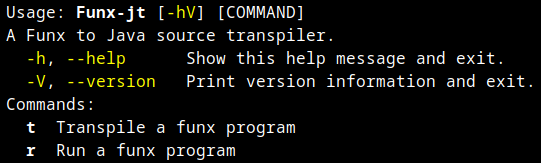
\includegraphics[width=\linewidth]{funx-jt-h.png}
        \vspace{2mm}
    \end{minipage}
    \begin{minipage}{0.85\textwidth}
        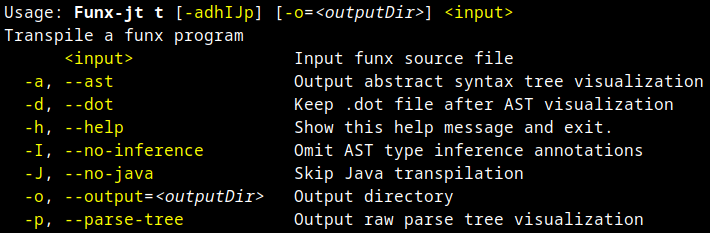
\includegraphics[width=\linewidth]{funx-jt-t-h.png}
        \vspace{2mm}
    \end{minipage}
    \begin{minipage}{0.85\textwidth}
        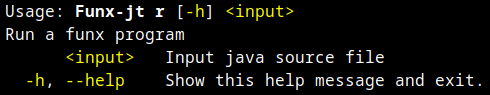
\includegraphics[width=\linewidth]{funx-jt-r-h.png}
    \end{minipage}
    \caption{Possibili comandi e opzioni della \textit{CLI}}
    \label{fig:5-compiler-cli}
\end{figure}

\newpage

\section{ANTLR}
\label{sec:5-1-antlr}

Al fine di semplificare lo sviluppo di \textit{lexer} e \textit{parser} per il linguaggio funzionale ideato
è stato scelto il generatore di \textit{parser} chiamato \texttt{ANTLR}%
\footnote{ANother Tool for Language Recognition,
    \citetitle{Parr-1995-ANTLRGenerator}, \cite{Parr-1995-ANTLRGenerator},
    \citetitle{Parr-2013-DefinitiveANTLR}, \cite{Parr-2013-DefinitiveANTLR}
    and ANTLRv4 (\url{https://www.antlr.org})}.

\noindent Grazie a tale strumento il processo iterativo di creazione della grammatica di \textbf{Funx}
è stato notevolmente semplificato e accelerato, in quanto \texttt{ANTLR} mette a disposizione del programmatore
un linguaggio per definire uno o più file di specifica per lessico e sintassi
(directory \texttt{Funx-jt/src/main/antlr} nel repository): questi vengono poi processati
per generare il codice sorgente del \textit{lexer} e del \textit{parser}.

\newpage

\subsection{Analisi lessicale}
\label{sec:5-2-lexical-analysis}

Data la probabile complessità delle regole della grammatica di \textbf{Funx}, fin dall'inizio la definizione dei \textit{token} (lessemi)
del linguaggio è stata separata dalla specifica del \textit{parser}.

\noindent Il file \texttt{FunxLexer.g4} descrive i lessemi dividendoli nelle seguenti cateogorie:
\begin{enumerate}
    \item \textit{whitespace}: caratteri di spaziatura e tabulazione;
    \item \textit{comments}: commenti di linea e blocco;
    \item \textit{keywords}: parole chiave del linguaggio;
    \item \textit{Java keywords}: parole chiave del linguaggio Java, da evitare;
    \item \textit{types}: tipi di dato (funzioni di tipo con arità 0);
    \item \textit{literals}: costanti booleane e numeriche;
    \item \textit{variables}: identificatori per variabili di tipo o nomi di funzioni;
    \item \textit{module}: identificatori il modulo;
    \item vari operatori simbolici per:
          \begin{itemize}
              \item \textit{bool}: valori booleani;
              \item \textit{comparison}: confronti tra numeri;
              \item \textit{arithmetic}: operazioni aritmetiche;
              \item \textit{other symbols}: simboli della sintassi (come \texttt{->}) e varie funzioni di libreria;
              \item \textit{delimiters}: parentesi tonde, quadre e graffe.
          \end{itemize}
\end{enumerate}

\noindent Le categorie 1 e 2 contengono token da scartare, tranne \texttt{NEWLINE}, mentre la categoria 4 è utile
qualora eventualmente si permetta allo sviluppatore di utilizzare tali parole chiave riservate,
effettuando una rinomina automatica; le categorie 7 e 8 devono necessariamente apparire dopo le categorie 3 e 4,
poiché tra \textit{keyword} e identificatori di ogni genere le prime devono avere la precedenza
(la posizione della categoria 5 tiene conto di una possibile futura estensione per consentire la creazione di nuovi tipi).


Oltre alle categorie illustrate, in testa al file sono presenti dei cosiddetti \textit{fragment} (frammenti)
che semplificano le espressioni regolari dei \textit{token} e complessivamente aumentano la leggibilità della specifica.

\newpage

\begin{lstlisting}[caption={Alcune \textit{token} del \textit{lexer}}, style=antlrCode, label={lst:5-2-lexer-antlr}]
lexer grammar FunxLexer;

// Fragments
fragment LALPHA: [a-z];
fragment UALPHA: [A-Z];
fragment ALPHA: LALPHA | UALPHA;
fragment ALPHA_: ALPHA | UnderScore;

fragment DIGIT: [0-9];
fragment DECIMAL: DIGIT+;

// Whitespace
NEWLINE: '\r'? '\n' | '\r';

TAB: [\t]+ @-> skip;
WS: [\u0020\u00a0\u1680\u2000\u200a\u202f\u205f\u3000]+ @-> skip;

// Comments
CloseMultiComment: '\./';
OpenMultiComment: '/\.';
SingleComment: '//';

COMMENT: SingleComment ~[\r\n]* @-> skip;
MULTICOMMENT: OpenMultiComment .*? CloseMultiComment @-> skip;

// Keywords
ELSE: 'else';
FI: 'fi';
IF: 'if';
IN: 'in';
LET: 'let';

// Java keywords
RESERVED_JAVA_KEYWORD: 'abstract' | 'assert' | 'boolean' | 'break' | 'byte' | [\.\.\.];

// Types
TYPE: BOOLTYPE | INTTYPE;
BOOLTYPE: 'Bool';

// Literals
INT: DECIMAL | OpenParen '\-' DECIMAL CloseParen;

// Variables
VARID: LALPHA (ALPHA_ | DIGIT)*;

// Module
MODULEID: UALPHA (ALPHA_ | DIGIT)*;

// Bool
And: '&&';
Not: '!!';

// Comparison
EqualsEquals: '\=\=';
NotEquals: '!\=';

// Arithmetic
Add: '\+';

// Other symbols
UnderScore: '_';
Arrow: '\-\>';

// Delimiters
OpenParen: '\(';
CloseParen: '\)';
\end{lstlisting}

\subsection{Analisi sintattica}
\label{sec:5-3-syntactic-analysis}

Il file \texttt{FunxParser.g4} contiene le regole concrete della grammatica di \textbf{Funx}:
nonostante la somiglianza con le grammatiche delle Figure~\ref{fig:2-funx-syntax} e \ref{fig:3-system-hm},
è evidente che queste non collimino esattamente a causa di zucchero sintattico e requisiti di \texttt{ANTLR}.

\noindent Lo strumento utilizzato, infatti, è un generatore di \textit{parser} di tipo \textit{top-down}
per grammatiche \textit{LL}, le quali in generale non supportano regole ricorsive a sinistra.

\noindent Essendo tali regole spesso comuni nella definizione di qualsiasi linguaggio di programmazione,
\textbf{Funx} incluso, \texttt{ANTLRv4} offre un diverso tipo di parsing, detto \textit{Adaptive LL(*)}%
\footnote{\citetitle{Parr-2011-FoundationANTLR}, \cite{Parr-2011-FoundationANTLR}
    and \citetitle{Parr-2014-AdaptiveLL}, \cite{Parr-2014-AdaptiveLL}}:
quest'ultimo è in grado di riscrivere automaticamente le grammatiche, eliminando la ricorsione a sinistra diretta (e.g. linee 36 e 38-43),
così da non incorrere in regole ambigue che potrebbero causare \textit{backtracking} e conseguente \textit{overhead}.

\noindent Il Codice~\ref{lst:5-parser} riporta integralmente le regole concrete della sintassi di \textbf{Funx}, tra cui:
\begin{itemize}
    \item \textit{module}: nome del modulo, funzione \texttt{main} opzionale e dichiarazioni globali;
    \item \textit{main}: funzione \texttt{main}, diversa dalle dichiarazioni classiche per l'assenza di schema di tipo e parametri lambda;
    \item \textit{declaration}: funzione con nome, tipo e parametri (e opzionalmente \texttt{with} per funzioni locali);
    \item \textit{typeElems}: tipo di una funzione, definito ricorsivamente secondo la grammatica del sistema di tipo di \textbf{Funx};
    \item \textit{statement}: per evitare ricorsione a sinistra indiretta, la separazione tra \textit{statement} e \textit{expression}
          forza l'uso di parentesi nei casi in cui lambda astrazioni, let e if siano usati all'interno di un'espressione;
    \item \textit{expression}: racchiude l'applicazione funzionale, tutte le regole relative agli operatori simbolici,
          specificandone la priorità implicite (Tabella~\ref{tab:2-sugar}), e le espressioni primarie
          (costanti, variabili e parentesi per controllare la precedenza);
    \item \textit{lambda, let, it}: corrispondenti alle produzioni per astrazione, let e if della grammatica formale.
\end{itemize}

\newpage

\begin{lstlisting}[caption={Grammatica per il \textit{parser}}, style=antlrCode, label={lst:5-parser}]
parser grammar FunxParser;
options { tokenVocab = FunxLexer; }

// Module
module: (MODULE MODULEID (Dot MODULEID)* NEWLINE+)?
    (main NEWLINE+)? declarations EOF;

declarations: declaration (NEWLINE declaration?)*;

main: id = MAIN Equals statement with?;

// Declaration
declaration: (declarationScheme NEWLINE)?
    id = VARID lambdaParams? Equals statement with?;

declarationScheme: id = VARID Colon typeElems;

with: NEWLINE WITH localDeclarations OUT;

localDeclarations: NEWLINE declarations NEWLINE;

// Type
typeElems: OpenParen typeElems CloseParen %# parenType%
    | VARID %# typeVar%
    | TYPE %# namedType%
    | <assoc = right> typeElems Arrow typeElems %# arrowType%;

// Statement
statement: expression %# expressionStatement%
    | lambda %# lambdaStatement%
    | let %# letStatement%
    | ifS %# ifStatement%;

// Expression
expression: primary %# primExpression%
    | expression expression %# appExpression%
    | <assoc = right> expression bop = Dot expression %# composeExpression%
    | expression bop = (Divide | Modulo | Multiply) expression %# divModMultExpression%
    | expression bop = (Add | Subtract) expression %# addSubExpression%
    | expression
        bop = (GreaterThan | GreaterThanEquals | LessThan | LessThanEquals)
        expression %# compExpression%
    | expression bop = (EqualsEquals | NotEquals) expression %# eqExpression%
    | uop = Not expression %# notExpression%
    | <assoc = right> expression bop = And expression %# andExpression%
    | <assoc = right> expression bop = Or expression %# orExpression%
    | <assoc = right> expression bop = Dollar expression %# rightAppExpression%;

primary: OpenParen statement CloseParen %# parenPrimary%
    | constant %# constPrimary% | VARID %# varPrimary%;

// Lambda
lambda: Backslash lambdaParams? Arrow statement;

lambdaParams: VARID+;

// Let
let: LET localDeclarations IN statement;

// If
ifS: IF statement THEN statement ELSE statement FI;

// Constant
constant: BOOL | numConstant;

numConstant: INT;    
\end{lstlisting}

\section{Albero sintattico astratto}
\label{sec:5-4-abstract-syntax-tree}

Il \textit{parser} generato da \texttt{ANTLR} utilizza i token identificati dal \textit{lexer} per costruire
un albero di parsing concreto (\textit{CST, concrete syntax tree}), molto complesso e poco comprensibile.
È dunque opportuno astrarre i dettagli del parsing in una struttura più semplice e facile da interpretare,
che rispecchia precisamente la grammatica del linguaggio (Figura~\ref{fig:2-funx-syntax}).
Tale operazione è effettuata dalla grande maggioranza dei compilatori moderni e il risultato è chiamato
\textbf{AST}, \textit{abstract syntax tree} (albero sintattico astratto).

\subsection{Gerarchia delle classi}
\label{sec:5-5-class-hierarchy}

Il primo passo per la costruzione di un \textbf{AST} per la sintassi di \textbf{Funx} è la definizione
di una gerarchia di classi \texttt{Java} che rappresentano i nodi dell'albero
(package \texttt{com.github.massimopavoni.funx.jt.ast.node}).


La classe astratta \texttt{ASTNode} è la radice dell'ordinamento poiché sarà usata per gli oggetti creati
a partire dal \textit{CST}: contiene la proprietà \texttt{inputPosition} per facilitare la segnalazione di errori
e vincola le classi figlie all'implementazione del metodo astratto \texttt{accept} per visitare i nodi.

\noindent Un'altra classe astratta, derivata dalla precedente, è \texttt{Expression}, la quale identifica
un'espressione ed è dotata di alcuni campi e metodi utili all'inferenza di tipo.


Ogni altra sottoclasse (ad eccezione di \texttt{Declarations}, utilizzata per dichiarazioni globali e locali)
è una trascrizione in \texttt{Java} delle produzioni della grammatica formale:
\begin{itemize}
    \item \texttt{Module}: modulo del programma;
    \item \texttt{Declaration}: dichiarazione di funzione;
    \item \texttt{Constant}: termini costanti;
    \item \texttt{Variable}: simboli per variabili;
    \item \texttt{Application}: applicazione di funzione;
    \item \texttt{Lambda}: astrazione per le funzioni anonime;
    \item \texttt{Let}: contenitore di dichiarazioni locali;
    \item \texttt{If}: costrutto condizionale.
\end{itemize}

\newpage

\begin{figure}
    \begin{tikzpicture}
        % classes
        \umlsimpleclass[type=abstract]{ASTNode}
        \umlsimpleclass[x=-4]{InputPosition}
        \umlsimpleclass[x=4,type=interface]{Inferable}
        \umlsimpleclass[x=-4,y=-2]{Module}
        \umlsimpleclass[y=-2]{Declarations}
        \umlsimpleclass[x=4,y=-2,type=abstract]{Expression}
        \umlsimpleclass[x=-2,y=-4]{Constant}
        \umlsimpleclass[x=-2,y=-5.5]{Variable}
        \umlsimpleclass[x=-2,y=-7]{Application}
        \umlsimpleclass[x=-2,y=-8.5]{Lambda}
        \umlsimpleclass[x=-2,y=-10]{Let}
        \umlsimpleclass[x=-2,y=-11.5]{If}
        % relationships
        \umlinherit[geometry=-|-]{Module}{ASTNode}
        \umlinherit{Declarations}{ASTNode}
        \umlinherit[geometry=-|-]{Expression}{ASTNode}
        \umlimpl{Expression}{Inferable}
        \umlinherit[geometry=-|,anchor2=-160]{Constant}{Expression}
        \umlinherit[geometry=-|,anchor2=-149]{Variable}{Expression}
        \umlinherit[geometry=-|,anchor2=-118]{Application}{Expression}
        \umlinherit[geometry=-|,anchor2=-62]{Lambda}{Expression}
        \umlinherit[geometry=-|,anchor2=-31]{Let}{Expression}
        \umlinherit[geometry=-|,anchor2=-20]{If}{Expression}
    \end{tikzpicture}
    \caption{Diagramma semplificato delle classi dell'\textbf{AST}}
    \label{fig:5-ast-classes}
    \vspace{4mm}
\end{figure}

\begin{lstlisting}[caption={Esempio di classe della gerarchia}, style=javaCode, label={lst:5-ast-class-java}]
public static final class Lambda extends Expression {
    public final String paramId;
    public final Expression expression;

    public Lambda(InputPosition inputPosition, String paramId, ASTNode expression) {
        super(inputPosition); // ASTNode constructor
        this.paramId = paramId;
        this.expression = (Expression) expression;
    }

    @Override // from Inferable interface
    public Utils.Tuple<Substitution, Type> infer(Context ctx) { ... }

    @Override // from Expression abstract class
    protected void propagateSubstitution(Substitution substitution) { ... }

    @Override // from ASTNode abstract class
    public @<T@> T accept(ASTVisitor@<? extends T@> visitor) {
        return visitor.visitLambda(this);
    }
}
\end{lstlisting}



\newpage

\subsection{AST builder}
\label{sec:5-6-ast-builder}

\texttt{ANTLR} offre due diversi approcci per analizzare l'albero di parsing:
\begin{itemize}
    \item \textit{listener}: i metodi implementati per l'analisi dei nodi sono chiamati seguendo la ricerca
          in profondità (\textit{DFS, depth-first search});
    \item \textit{visitor}: i nodi possono essere visitati arbitrariamente tramite il metodo \texttt{visit},
          senza seguire un ordine specifico; non tutti i metodi devono essere implementati
          ed è possibile ignorare dei nodi o ri-visitarli.
\end{itemize}

\noindent La seconda opzione è indubbiamente più versatile, e può essere per esempio anche utilizzata
qualora si desideri evitare completamente la costruzione di un \textbf{AST} e chiamare i metodi di visita
per eseguire il codice (e.g. linguaggi interpretati).

\noindent Nel caso di \textbf{Funx-jt} la scelta ricade appunto sul \textit{visitor} in virtù
della probabilità di dover "saltare" alcuni nodi e ottenerne direttamente le informazioni interne.

\noindent Durante la compilazione del progetto \texttt{Java}, \texttt{Gradle} è configurato per generare
le seguenti classi nel package \texttt{com.github.massimopavoni.funx.jt.parser}:
\begin{itemize}
    \item \texttt{FunxLexer}: \textit{lexer};
    \item \texttt{FunxParser}: \textit{parser};
    \item \texttt{FunxParserVisitor}: interfaccia generica per differenti implementazioni del \textit{visitor}
          (estende l'interfaccia \texttt{ParseTreeVisitor} di \texttt{ANTLR});
    \item \texttt{FunxParserBaseVisitor}: classe predefinita che percorre l'intero albero di parsing
          (estende la classe astratta \texttt{AbstractParseTreeVisitor} per ereditare alcuni metodi standard come \texttt{visitChildren}).
\end{itemize}

\noindent La classe \texttt{ASTBuilder} estende a sua volta \texttt{FunxParserBaseVisitor} e sovrascrive quasi tutti i metodi ereditati;
in particolare, \texttt{ASTBuilder} effettua la composizione degli schemi di tipo definiti dall'utente (sezione~\ref{sec:5-8-system-hm})
e l'eliminazione dello zucchero sintattico mediante l'uso di alcune proprietà e metodi ausiliari.


Inoltre, all'interno del package \texttt{com.github.massimopavoni.funx.jt.ast} viene definita una classe enumeratore,
\texttt{PreludeFunction} contenente le funzioni di libreria standard, con i relativi simboli e gli schemi di tipo corrispondenti.

\vspace{4mm}
\begin{lstlisting}[caption={Parte del codice di \texttt{PreludeFunction}}, style=javaCode, label={lst:5-preludefunction-java}]
public enum PreludeFunction {
    COMPOSE(".", "compose",
        new Scheme(Set.of(0L, 1L, 2L),
            arrowOf(arrowOf(ZERO, ONE), arrowOf(TWO, ZERO), TWO, ONE)), false);

    public final String symbol;
    public final String id;
    public final Scheme scheme;
    public final boolean nativeJava;

    PreludeFunction(String symbol, String id,
        Scheme scheme, boolean nativeJava) { ... }

    public static PreludeFunction fromSymbol(String symbol) {
        return Utils.enumFromField(PreludeFunction.class,
            f @-> f.symbol.equals(symbol));
    }
}
\end{lstlisting}

\newpage

\begin{lstlisting}[caption={Metodi per astrazioni annidate e operatori simbolici binari}, style=javaCode, label={lst:5-auxiliary-methods-java}]
@Override
private ASTNode createLambdaChain(
        InputPosition position, Deque@<String@> params, ASTNode expression) {
    if (params.size() == 1)
        return new Expression.Lambda(
            position,
            params.getFirst(),
            expression);
    return new Expression.Lambda(
        position,
        params.pop(),
        createLambdaChain(position, params, expression));
}

@Override
private ASTNode binarySymbolApplication(
        InputPosition position, String symbol, ASTNode left, ASTNode right) {
    return new Expression.Application(
        position,
        new Expression.Application(
                position,
                new Expression.Variable(
                        position,
                        PreludeFunction.fromSymbol(symbol).id),
                left),
        right);
}
\end{lstlisting}
\vspace{4mm}
\begin{lstlisting}[caption={Alcuni metodi \textit{visit} di \texttt{ASTBuilder}}, style=javaCode, label={lst:5-astbuilder-java}]
public class ASTBuilder extends FunxParserBaseVisitor@<ASTNode@> {
    @Override
    public ASTNode visitAppExpression(FunxParser.AppExpressionContext ctx) {
        return new Expression.Application(getInputPosition(ctx),
            visit(ctx.expression(0)), visit(ctx.expression(1)));
    }

    @Override
    public ASTNode visitComposeExpression(FunxParser.ComposeExpressionContext ctx) {
        return binarySymbolApplication(getInputPosition(ctx),
            Utils.fromLexerToken(ctx.bop.getType()),
            visit(ctx.expression(0)), visit(ctx.expression(1)));
    }
    
    @Override
    public ASTNode visitOrExpression(FunxParser.OrExpressionContext ctx) {
        // transform logical disjunction into if statement for lazy behavior
        return new Expression.If(getInputPosition(ctx),
            visit(ctx.expression(0)),
            new Expression.Constant(InputPosition.UNKNOWN, true),
            visit(ctx.expression(1)));
    }

    @Override
    public ASTNode visitLambda(FunxParser.LambdaContext ctx) {
        return createLambdaChain(getInputPosition(ctx),
            // lambda params are syntactic sugar for a lambda chain
            ctx.lambdaParams().VARID().stream().map(ParseTree::getText)
                .collect(Collectors.toCollection(ArrayDeque::new)),
                visit(ctx.statement()));
    }
}    
\end{lstlisting}

\newpage

\noindent Il codice del compilatore include una classe astratta \texttt{ASTVisitor} atta a permettere l'analisi
dell'\textbf{AST} in modo simile ai \textit{visitor} di \texttt{ANTLR}.
Il Codice~\ref{lst:5-ast-example-funx} e la Figura~\ref{fig:5-ast-example-debug-graphviz}
mostrano un \textbf{AST} come verrebbe creato da \texttt{ASTBuilder}; la \textit{CLI} sviluppata fornisce
delle opzioni per la visualizzazione dell'albero, generata utilizzando il software \texttt{Graphviz}%
\footnote{Graph Visualization Software (\url{https://graphviz.org})}
con un \textit{visitor} che costruisce progressivamente una stringa nel linguaggio \texttt{DOT}.

\vspace{4mm}
\begin{lstlisting}[caption={Programma in \textbf{Funx}}, style=funxCode, label={lst:5-ast-example-funx}]
tautology : Bool @-> Bool
tautology x = x || !!x
\end{lstlisting}

\begin{figure}
    \vspace{4mm}
    \begin{minipage}[c]{0.6\textwidth}
        \centering
        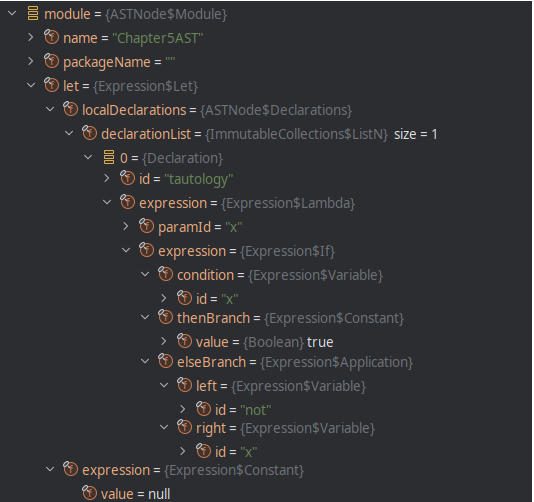
\includegraphics[width=\linewidth,height=\linewidth]{ast-example-debug.png}
    \end{minipage}%
    \hfill
    \begin{minipage}[c]{0.4\textwidth}
        \centering
        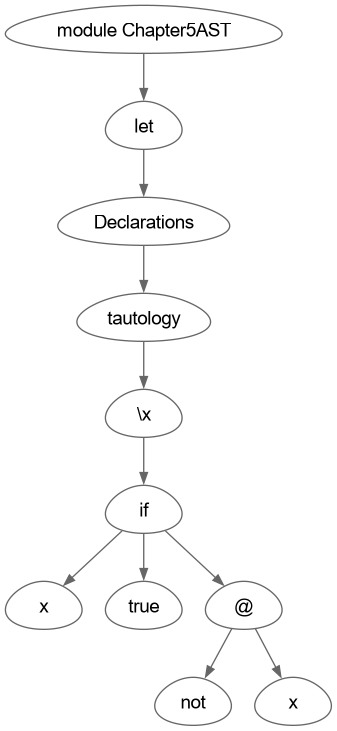
\includegraphics[width=0.8\linewidth]{ast-example-graphviz.png}
    \end{minipage}
    \caption{Oggetto \textbf{AST} in \textit{debug} e visualizzazione dell'albero}
    \label{fig:5-ast-example-debug-graphviz}
\end{figure}


\newpage

\section{Motore inferenziale}
\label{sec:5-7-inference-engine}

I sistemi di tipo e l'inferenza descritti nel Capitolo~\ref{chap:3-inference} costituiscono una parte imprescindibile del software,
data l'incapacità di simulare il polimorfismo parametrico del \textit{sistema HM} lasciando al compilatore \texttt{Java}
il compito d'inferire e controllare i tipi generici dei metodi (o classi).
In tal caso, infatti, la compilazione fallirebbe a causa di tipi "troppo generici" e \textit{type casting} non permesso
in maniera implicita (e.g. non si è in grado di conciliare un tipo generico con una lambda espressione).

\begin{figure}
    \vspace{4mm}
    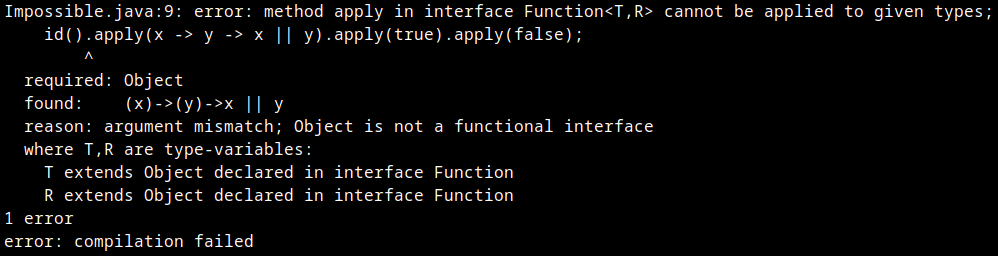
\includegraphics[width=\textwidth]{5-7-impossible-java.png}
    \caption{Esempio di errore in \texttt{Java} dovuto a tipi generici}
    \label{fig:5-7-impossible-java}
    \vspace{4mm}
\end{figure}

\noindent La linea di codice citata in Figura~\ref{fig:5-7-impossible-java} non è intrinsecamente errata,
ma non può essere compilata in mancanza d'informazioni riguardanti il parametro di tipo generico della funzione \texttt{id}
(con tipo di ritorno \texttt{Function<T, T>}): il problema da risolvere è quindi conoscere il tipo dell'espressione
in input alla prima chiamata del metodo \texttt{apply}.


Il motore inferenziale è la parte del compilatore che si occupa di stabilire i tipi delle espressioni seguendo le regole
d'inferenza e i passi dell'\textit{algoritmo $\mathcal{W}$} \cite{Grabmuller-2006-AlgorithmW}
descritti nella sezione~\ref{sec:3-4-hm-type-inference}; la fase d'inferenza avviene subito dopo parsing
e costruzione dell'\textbf{AST}, anticipando la generazione del codice \texttt{Java}.

\subsection{Sistema HM}
\label{sec:5-8-system-hm}

Seguendo la grammatica del sistema di tipo di \textbf{Funx} e similmente alla gerarchia per l'albero sintattico astratto,
l'implementazione del \textit{sistema HM} presenta le seguenti classi e sottoclassi:
\begin{itemize}
    \item \texttt{Scheme}: schemi di tipo;
    \item \texttt{Type}: classe astratta per i monotipi;
    \item \texttt{Error}: tipo errore per la continuazione dell'inferenza;
    \item \texttt{Boring}: tipo vuoto per costanti con valore \texttt{null};
    \item \texttt{Variable}: variabili di tipo;
    \item \texttt{FunctionApplication}: applicazione di funzione di tipo.
\end{itemize}

\newpage

\begin{figure}
    \begin{tikzpicture}
        % classes
        \umlsimpleclass[type=interface]{Types}
        \umlsimpleclass[x=-4,type=interface]{Inferable}
        \umlsimpleclass[x=4,type=enum]{TypeFunction}
        \umlsimpleclass[x=-3,y=-1.15]{Context}
        \umlsimpleclass[x=3,y=-1.15]{Substitution}
        \umlsimpleclass[x=-3,y=-2.2]{Scheme}
        \umlsimpleclass[x=3,y=-2.2,type=abstract]{Type}
        \umlsimpleclass[x=-1,y=-3.4,type=singleton]{Error}
        \umlsimpleclass[x=-1,y=-4.7,type=singleton]{Boring}
        \umlsimpleclass[x=-1,y=-5.85]{Variable}
        \umlsimpleclass[x=-1,y=-6.9]{FunctionApplication}
        % relationships
        \umlinherit[geometry=-|,anchor2=-145]{Context}{Types}
        \umlinherit[geometry=-|,anchor2=-35]{Substitution}{Types}
        \umlinherit[geometry=-|,anchor2=-117]{Scheme}{Types}
        \umlinherit[geometry=-|,anchor2=-63]{Type}{Types}
        \umlinherit[geometry=-|,anchor2=-145]{Error}{Type}
        \umlinherit[geometry=-|,anchor2=-116]{Boring}{Type}
        \umlinherit[geometry=-|,anchor2=-64]{Variable}{Type}
        \umlinherit[geometry=-|,anchor2=-35]{FunctionApplication}{Type}
    \end{tikzpicture}
    \caption{Diagramma semplificato delle classi del \textit{sistema HM}}
    \label{fig:5-8-hm-classes}
    \vspace{4mm}
\end{figure}

\begin{lstlisting}[caption={Esempio di sottoclasse di \texttt{Type}}, style=javaCode, label={lst:5-8-hm-class-java}]
public static final class Variable extends Type {
    public final long id;
    
    public Variable(long id) { this.id = id; }

    public static String toString(long id) {
        return id < 26 ? Character.toString((char) ('a' + id)) : "t" + id;
    }

    public static String toFancyString(long id) {
        return id < 24 ? Character.toString((char) (945 + id)) : "t" + id;
    }

    @Override
    public Set@<Long@> freeVariables() { ... }

    @Override
    public Type applySubstitution(Substitution substitution) { ... }
}
\end{lstlisting}
\vspace{4mm}

\noindent Altre classi e interfacce di supporto sono fondamentali per la definizione dei comportamenti precedentemente descritti:
\begin{itemize}
    \item \texttt{Types}: interfaccia per operazioni comuni negli oggetti che agiscono a stretto contatto con i tipi;
          specifica i metodi per il calcolo delle variabili libere e l'applicazione di una sostituzione;
    \item \texttt{Inferable}: interfaccia già visibile in Figura~\ref{fig:5-5-ast-classes} e che identifica i nodi
          dell'\textbf{AST} che implementano un metodo di inferenza (i.e. le sottoclassi di \texttt{Expression});
    \item \texttt{TypeFunction}: enumerazione delle funzioni di tipo disponibili;
    \item \texttt{Substitution}: lista di sostituzioni da variabili di tipo a monotipi;
    \item \texttt{Context}: contesto di inferenza con vincoli tra variabili e schemi di tipo.
\end{itemize}

\newpage

\begin{lstlisting}[caption={Interfacce utili nel \textit{sistema HM}}, style=javaCode, label={lst:5-8-hm-interfaces-java}]
package com.github.massimopavoni.funx.jt.ast.node;

public sealed interface Inferable permits Expression {
    Utils.Tuple@<Substitution, Type@> infer(Context ctx);
}

// ----------------

package com.github.massimopavoni.funx.jt.ast.typesystem;

sealed interface Types@<T extends Types@<T@>@>
        permits Type, Scheme, Substitution, Context {
    Set@<Long@> freeVariables();

    T applySubstitution(Substitution substitution);
}
\end{lstlisting}
\vspace{4mm}
\begin{lstlisting}[caption={Altre classi del \textit{sistema HM}}, style=javaCode, label={lst:5-8-hm-more-classes-java}]
public final class Context implements Types@<Context@> {
    private final Map@<String, Scheme@> environment;

    public Scheme bindingOf(String variable) {
        return environment.get(variable);
    }

    @Override
    public Set@<Long@> freeVariables() {
        return environment.values().stream().flatMap(s @-> s.freeVariables().stream())
            .collect(ImmutableSet.toImmutableSet());
    }

    @Override
    public Context applySubstitution(Substitution substitution) {
        Context newCtx = new Context(this);
        newCtx.environment.replaceAll((v, s) @-> s.applySubstitution(substitution));
        return newCtx;
    }
}

public final class Substitution implements Types@<Substitution@> {
    public static final Substitution EMPTY = new Substitution();
    private final Map@<Long, Type@> variableTypes;

    public Type substituteOf(Long variable) {
        return variableTypes.get(variable);
    }

    @Override
    public Set@<Long@> freeVariables() {
        // similar to Context
    }

    @Override
    public Substitution applySubstitution(Substitution substitution) {
        return new Substitution(variableTypes.entrySet().stream()
            .collect(Collectors.toMap(Map.Entry::getKey,
                e @-> e.getValue().applySubstitution(substitution))));
    }
}
\end{lstlisting}

\newpage

\subsection{Inferenza su espressioni}
\label{sec:5-9-expression-inference}

La classe \texttt{InferenceEngine} contiene solamente proprietà e metodi statici, e non adotta lo stesso
procedimento di esplorazione dell'albero sintattico delle classi figlie di \texttt{ASTVisitor}
(visualizzazione e traduzione in \texttt{Java}): il cammino attraverso l'\textbf{AST} inizia con un metodo
di avvio per chiamate ricorsive sulle funzioni di inferenza di ciascun nodo,
a partire dal \texttt{let} delle dichiarazioni globali di un modulo.


Come già accennato nella sezione~\ref{sec:3-4-hm-type-inference}, i metodi sono molto simili all'\textit{algoritmo $\mathcal{W}$} mostrato,
e le classi ausiliarie appena descritte facilitano lo sviluppo delle funzioni di inferenza seguendo tale modello da vicino.

\noindent Ciò nonostante, si vuol descrivere brevemente l'implementazione del metodo \texttt{infer} della classe \texttt{Let},
in quanto di particolare interesse per le modifiche apportate al fine di consentire mutua ricorsione tra funzioni polimorfe.

\noindent L'inferenza per \texttt{let}, presentata nel Codice~\ref{lst:5-9-let-inference-java}, si divide in 4 fasi:
\begin{itemize}
    \item linee 3-21, inizializzazione del contesto:
          \begin{itemize}
              \item creazione di una mappa per le posizioni delle dichiarazioni;
              \item copia del contesto originale;
              \item controllo di dichiarazioni duplicate;
              \item aggiornamento del contesto con schemi di tipo temporanei;
          \end{itemize}
    \item linee 23-43, inferenza sulle dichiarazioni locali:
          \begin{itemize}
              \item initializzazione della sostituzione;
              \item inferenza per ogni dichiarazione;
              \item unificazione tra tipi noti (compresi quelli temporanei) e tipi inferiti, progressiva composizione delle sostituzioni;
              \item applicazione della sostituzione al contesto;
          \end{itemize}
    \item linee 45-53, generalizzazione dei tipi:
          \begin{itemize}
              \item propagazione delle sostituzioni e chiamata alla funzione \texttt{generalize};
              \item controllo del tipo definito dallo sviluppatore;
              \item aggiornamento del contesto;
          \end{itemize}
    \item linee 55-60, inferenza sull'espressione principale:
          \begin{itemize}
              \item chiamata ricorsiva;
              \item composizione finale delle sostituzioni;
              \item propagazione delle sostituzioni e assegnamento del tipo per il nodo \texttt{let}.
          \end{itemize}
\end{itemize}

\newpage

\begin{lstlisting}[caption={Metodo di inferenza per espressioni \texttt{let}}, style=javaCode, label={lst:5-9-let-inference-java}]
@Override
public Utils.Tuple@<Substitution, Type@> infer(Context ctx) {
    // check for duplicate declarations within the same let
    Map@<String, InputPosition@> declarationPositions = new HashMap@<@>();

    Context newCtx = new Context(ctx);

    for (Declaration decl : localDeclarations.declarationList) {
        if (declarationPositions.containsKey(decl.id))
            InferenceEngine.reportError(decl.inputPosition,
                String.format("variable '%s' already declared at %s",
                    decl.id, declarationPositions.get(decl.id)));
        else {
            declarationPositions.put(decl.id, decl.inputPosition);

            // while also updating the context with placeholder schemes,
            // so that self and mutual recursion can be handled
            newCtx.bind(decl.id,
                new Scheme(Collections.emptySet(), InferenceEngine.newTypeVariable()));
        }
    }

    // proceed to infer all local declarations
    Substitution subst = Substitution.EMPTY;

    for (Declaration decl : localDeclarations.declarationList) {
        Utils.Tuple@<Substitution, Type@> declInference = decl.expression.infer(newCtx);
        try {
            // unifying types of known bindings,
            // gradually composing substitutions and updating context
            subst = subst.compose(declInference.fst())
                .compose(newCtx.bindingOf(decl.id).type
                    .applySubstitution(subst)
                    .unify(declInference.snd())); // could throw TypeException

            decl.expression.type = declInference.snd().applySubstitution(subst);

            newCtx = newCtx.applySubstitution(subst);
        } catch (TypeException e) {
            InferenceEngine.reportError(decl.inputPosition, e.getMessage());
            decl.expression.type = Type.Error.INSTANCE;
        }
    }

    // finally generalize all types and check against actual user-defined schemes
    for (Declaration decl : localDeclarations.declarationList) {
        decl.expression.propagateSubstitution(subst);

        Scheme expectedScheme = decl.expression.type.generalize(ctx);
        decl.checkScheme(expectedScheme, ctx);

        newCtx.bind(decl.id, decl.scheme());
    }

    // now it's possible to infer the expression type
    Utils.Tuple@<Substitution, Type@> exprInference = expression.infer(newCtx);

    subst = subst.compose(exprInference.fst());
    type = exprInference.snd().applySubstitution(subst);
    expression.propagateSubstitution(subst);

    return new Utils.Tuple@<@>(subst, type);
}
\end{lstlisting}

\newpage

\begin{lstlisting}[caption={Esempio di inferenza}, style=funxCode, label={lst:5-9-types-funx}]
main = countdown 1825

countdown : Int @-> Int
countdown = until (equalsEquals 0) (flip subtract 1) 

until p f = until1
    with
        until1 x = if p x then x else until1 (f x) fi
    out    
\end{lstlisting}

\begin{figure}
    \vspace{4mm}
    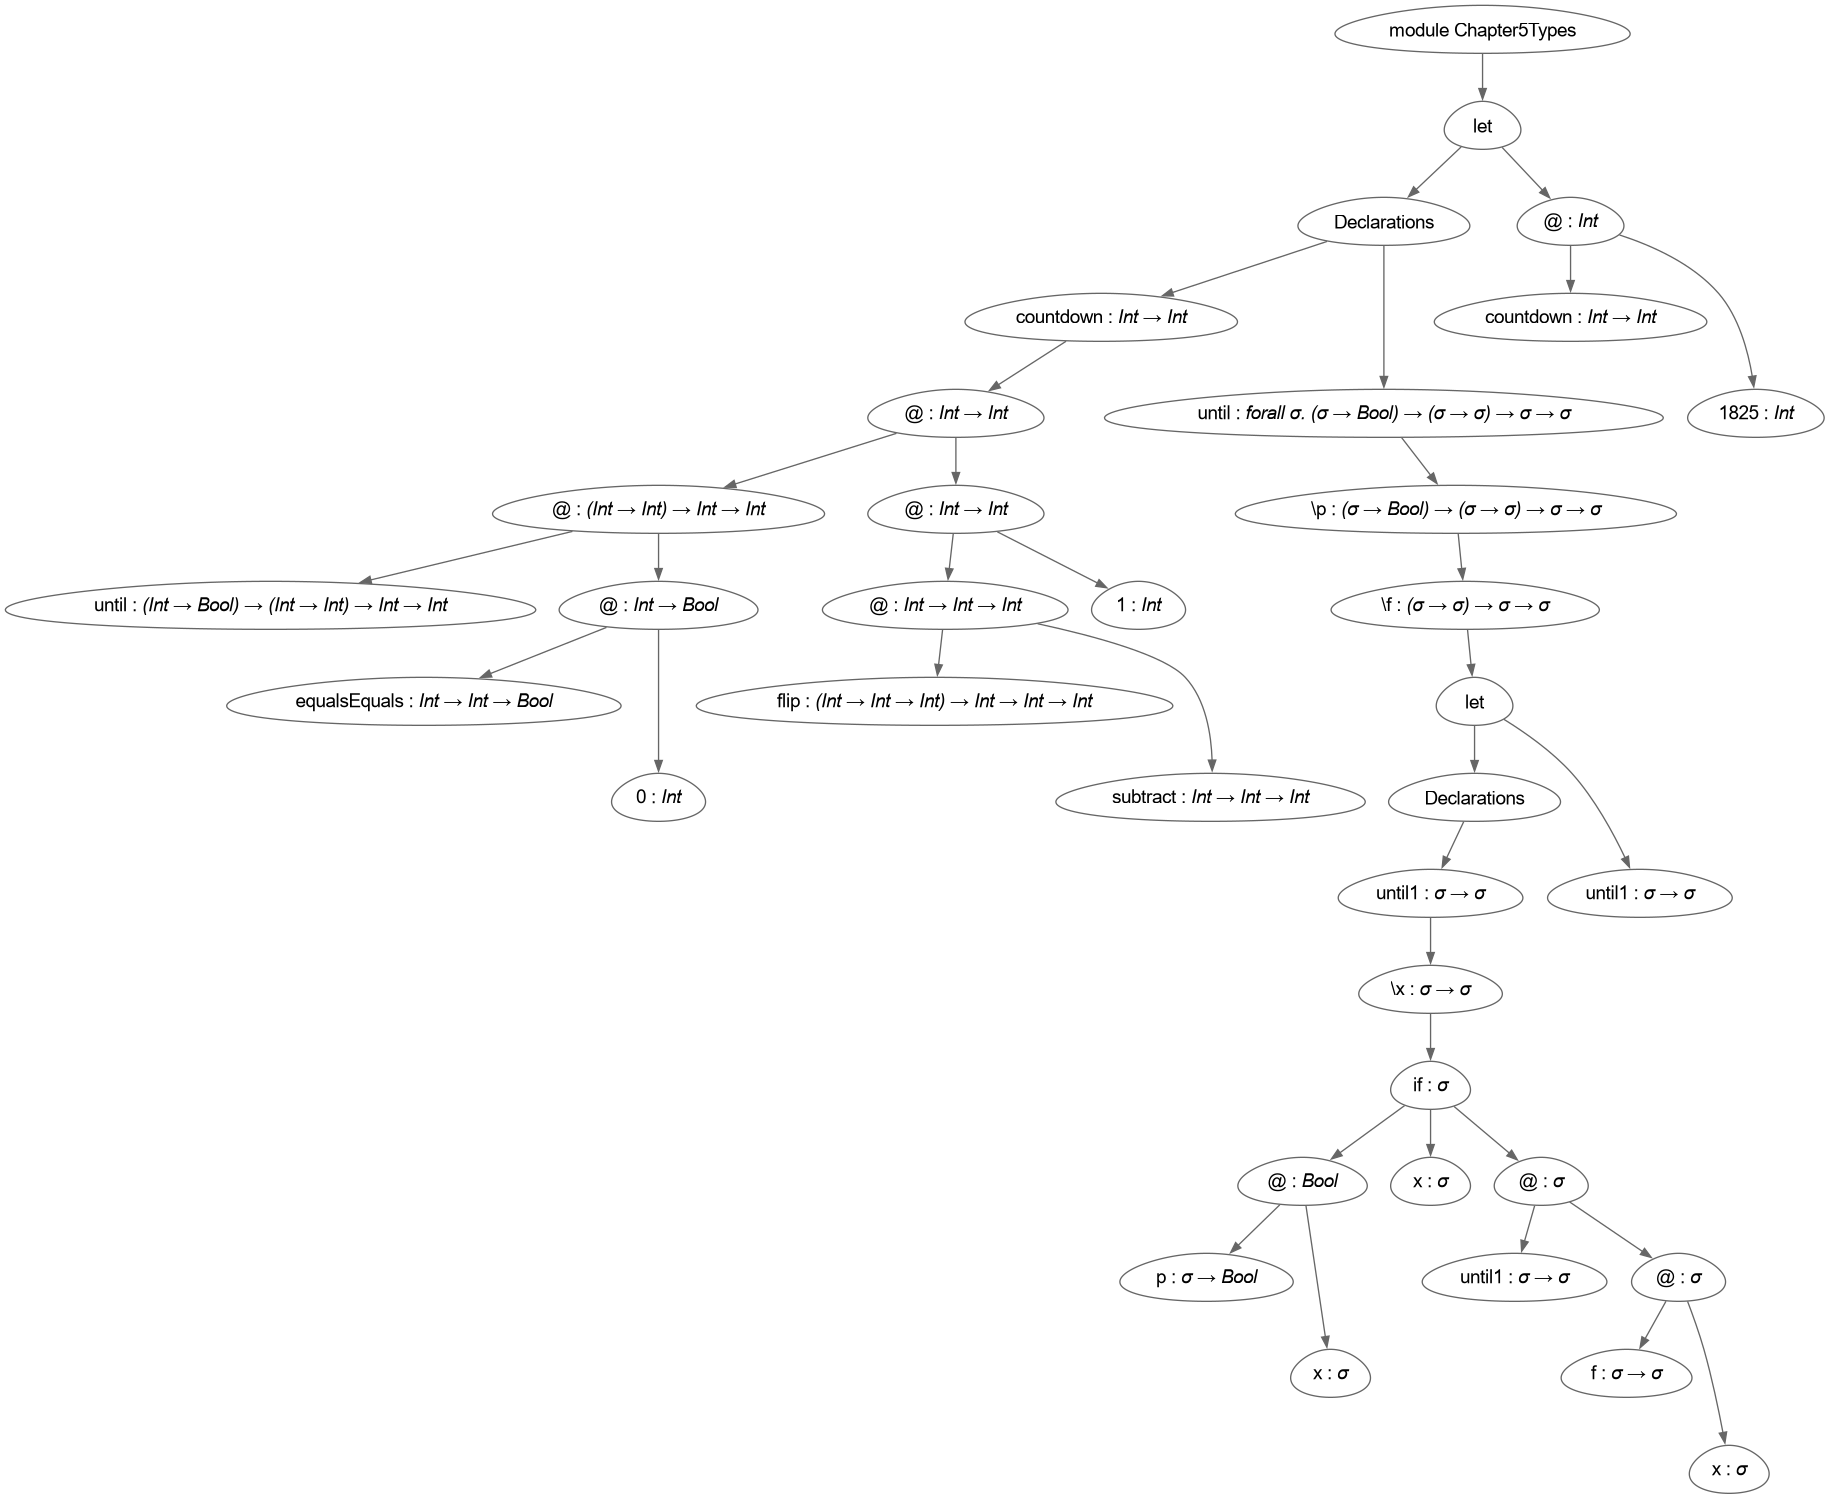
\includegraphics[width=\textwidth]{5-9-type-annotations.png}
    \caption{\textbf{AST} con annotazioni di tipo}
    \label{fig:5-9-type-annotations}
\end{figure}


\section{Traduzione in Java}
\label{sec:5-10-java-translation}

La sottoclasse più importante di \texttt{ASTVisitor} è \texttt{JavaTranspiler}, il \textit{visitor} che si occupa
dell'ultimo stadio di compilazione, la traduzione dell'\textbf{AST} in codice \texttt{Java}:
come per \texttt{GraphvizBuilder}, la classe compone una stringa
che rappresenta il programma \texttt{Java} corrispondente al codice \textbf{Funx} sorgente.


Avendo già illustrato degli esempi di traduzione nel Capitolo~\ref{chap:4-java}, in questa sezione si
discuteranno le scelte e i compromessi nel processo di traduzione, e il modo in cui le limitazioni
di \texttt{Java} possano essere talvolta aggirate "piegando" le regole.

\subsection{Membri statici}
\label{sec:5-11-static-members}

Il paradigma dichiarativo dei linguaggi funzionali è ben diverso dalla programmazione ad oggetti di molti altri linguaggi rinomati,
motivo per cui la scelta di tradurre ogni programma \textbf{Funx} in un'unica classe statica è vista come semplice soluzione
per evitare complicanze e \textit{overhead} per la creazione di oggetti in aggiunta alle \texttt{Function}.


Ogni funzione definita diviene perciò una proprietà statica della classe in caso di monotipi (sezione~\ref{sec:5-13-monomorphic-declarations})
o un metodo statico con parametri di tipo in caso di politipi (sezione~\ref{sec:5-14-polymorphic-functions-instantiation}),
mentre scrittura della classe stessa inizia con \textit{import} statici delle funzioni di libreria standard e un costruttore privato.

\vspace{4mm}
\begin{lstlisting}[caption={Prime aggiunte alla stringa \texttt{Java}}, style=javaCode, label={lst:5-11-first-append-java}]
// append package, imports, class declaration and constructor

builder.append(module.packageName.isEmpty()
        @? ""
        @: String.format("package %s;%n", module.packageName.toLowerCase()))
    .append("\n\nimport ").append(Function.class.getName())
    .append(";\n\nimport ").append(JavaPrelude.class.getName())
    .append(";\n\nimport ").append(FunxPrelude.class.getName())
    .append(";\n\nimport static ").append(JavaPrelude.class.getName())
    .append(".*;\nimport static ").append(FunxPrelude.class.getName())
    .append(".*;\n\npublic class ").append(module.name).append(" {\n")
    .append("private ").append(module.name)
    .append("() {\n// private constructor to prevent instantiation\n}\n\n");
\end{lstlisting}
\vspace{4mm}
\begin{lstlisting}[caption={Corrispondente codice \texttt{Java} generato}, style=javaCode, label={lst:5-11-class-start-java}]
import java.util.function.Function;

import com.github.massimopavoni.funx.lib.JavaPrelude;

import com.github.massimopavoni.funx.lib.FunxPrelude;

import static com.github.massimopavoni.funx.lib.JavaPrelude.*;
import static com.github.massimopavoni.funx.lib.FunxPrelude.*;

public class Test {
    private Test() {
        // private constructor to prevent instantiation
    }    
\end{lstlisting}

\newpage

\subsection{Stack dei contesti}
\label{sec:5-12-scope-stack}

Durante l'esplorazione dell'\textbf{AST} è necessario tenere traccia dello \textit{scope}, il contesto, del quale le dichiarazioni
o i parametri lambda fanno parte: la soluzione adottata prevede l'uso di uno \textit{stack} contenente i contesti attivi,
rappresentati a loro volta da mappe (le variabili dichiarate sono le chiavi, le relative informazioni sono i valori).

\noindent Lo \textit{stack} dei contesti è in realtà implementato attraverso una lista, per via della necessità di iterare
su tutti i contesti e trovare una variabile richiesta (\textit{lookup}).

\vspace{4mm}
\begin{lstlisting}[caption={Struttura e metodi per lo \textit{scope}}, style=javaCode, label={lst:5-12-scope-stack-methods-java}]
private final List@<Map@<String, Utils.Tuple@<Scheme, String@>@>@>
    scopes = new ArrayList@<@>();

private void addToScope(List@<Declaration@> declarations, String scope) {
    scopes.addFirst(declarations.stream()
        .collect(ImmutableMap.toImmutableMap(
            decl @-> decl.id,
            decl @-> new Utils.Tuple@<@>(decl.scheme(), scope))));
}

private void addToScope(String id, Scheme scheme, String scope) {
    scopes.addFirst(Collections.singletonMap(id, new Utils.Tuple@<@>(scheme, scope)));
}
\end{lstlisting}
\vspace{4mm}
\begin{lstlisting}[caption={Aggiunta di contesto per modulo, lambda astrazioni e \texttt{let}}, style=javaCode, label={lst:5-12-lambda-let-scope-java}]
@Override
public Void visitModule(ASTNode.Module module) {
    // add Prelude functions to the scope
    scopes.addFirst(Arrays.stream(PreludeFunction.values())
        .collect(ImmutableMap.toImmutableMap(
            pf @-> pf.id,
            pf @-> new Utils.Tuple@<@>(pf.scheme, pf.nativeJava
                @? JavaPrelude.class.getSimpleName()
                @: FunxPrelude.class.getSimpleName()))));
    // add module functions to the scope
    addToScope(module.let.localDeclarations.declarationList, module.name);
    // ...
    scopes.removeFirst();
    return null;
}

@Override
public Void visitLambda(Expression.Lambda lambda) {
    // add lambda parameter to the scope
    addToScope(lambda.paramId, new Scheme(Collections.emptySet(),
        ((Type.FunctionApplication) lambda.type()).arguments.getFirst()), null);
    // ...
    scopes.removeFirst();
    return null;
}

@Override
public Void visitLet(Expression.Let let) {
    currentLevel++;
    // add let local declarations to the scope
    addToScope(let.localDeclarations.declarationList, "this");
    // ...
    // restore previous scope state and level
    scopes.removeFirst();
    currentLevel--;
    return null;
}
\end{lstlisting}

\newpage

\noindent Nei Codici~\ref{lst:5-12-scope-stack-methods-java}~e~\ref{lst:5-12-lambda-let-scope-java} sono mostrate:
\begin{itemize}
    \item la lista dei contesti e le funzioni per la loro gestione: le tuple assegnate ai nomi delle dichiarazioni di uno \textit{scope}
          conservano lo schema di tipo e il nome della classe in cui la variabile è definita
          (\texttt{JavaPrelude}, \texttt{FunxPrelude}, nome del modulo creato,
          \texttt{null} per parametri lambda e \texttt{this} per i \texttt{let});
    \item l'aggiunta dei contesti per \texttt{Module}, \texttt{Lambda} e \texttt{Let}, rispettivamente:
          funzioni di libreria e dichiarazioni del modulo stesso, parametro lambda,
          dichiarazioni locali con l'incremento del livello di annidamento.
\end{itemize}

\subsection{Dichiarazioni monomorfe}
\label{sec:5-13-monomorphic-declarations}

La possibilità in \textbf{Funx} di utilizzare funzioni ricorsive e mutuamente ricorsive
e la volontà di evitare la traduzione di ogni dichiarazione in un metodo sono in conflitto
a causa di \textit{Illegal Self Reference} e \textit{Illegal Forward Reference}:
tali errori si presentano durante la compilazione del codice \texttt{Java}
qualora i campi statici che identificano funzioni monomorfe vengano dichiarati e inizializzati
nello stesso \textit{statement} (stessa linea).


La dichiarazione delle proprietà deve avvenire prima di poter apparire nell'inizializzazione di altre variabili;
si potrebbe effettuare un'analisi iniziale dell'\textbf{AST} per identificare le dipendenze tra le funzioni
(approccio di ordinamento topologico estremamente utile anche per l'inferenza), ma la soluzione adottata
è di più semplice implementazione.


Come si può notare nel Codice~\ref{lst:5-13-monomorphic-java} e in alcuni esempi già presentati in precedenza,
si effettua la dichiarazione di ogni campo, pubblico e statico per le dichiarazioni globali, privato per quelle locali,
e solo successivamente si inizializzano rispettivamente con blocco statico e metodo \texttt{eval}.

\vspace{4mm}
\begin{lstlisting}[caption={Traduzione di funzioni monomorfe}, style=javaCode, label={lst:5-13-monomorphic-java}]
public class Chapter5Monomorphic {
    private Chapter5Monomorphic() {
        // private constructor to prevent instantiation
    }
    
    public static void main(String[] args) {
        System.out.println(add.apply(add.apply(fun1).apply(fun2)).apply(letFun));
    }
    
    public static Long fun1;    
    public static Long fun2;    
    public static Long letFun;
    
    static {
        fun1 = 1L;    
        fun2 = 2L;    
        letFun =
            (new Let@<@>() {
                private Long a;    
                private Long b;
    
                @Override
                public Long _eval() {
                    a = 3L;
                    b = 4L;
                    return add.apply(a).apply(b);
                }
            })._eval();
    }
}
\end{lstlisting}

\newpage

\noindent Poiché potrebbero essere presenti diversi \texttt{let} annidati, è necessario tenere traccia delle espressioni
corpo delle dichiarazioni monomorfe in modo da poterle inizializzare al momento corretto, dopo aver tradotto ulteriori classi interne.

\noindent La procedura di traduzione di dichiarazioni monomorfe si compone delle seguenti fasi:
\begin{itemize}
    \item definizione di uno \textit{stack} contenente mappe tra nomi delle dichiarazioni e nodi espressione corrispondenti;
    \item inserimento di una nuova mappa per il livello corrente di annidamento (modulo o espressione \texttt{let});
    \item inferenza delle funzioni globali o locali con dichiarazione delle variabili e aggiunta delle espressioni monomorfe
          alla mappa corrente (potrebbero essere aggiunti nuovi livelli prima di poterne "riempire" uno);
    \item creazione del blocco statico (o metodo \texttt{eval} per le espressioni \texttt{let}) con le inizializzazioni
          delle funzioni con monotipo: in questa fase finale torna utile la versatilità del \textit{visitor pattern} per posticipare
          la traduzione delle espressioni.
\end{itemize}

\vspace{4mm}
\begin{lstlisting}[caption={Traduzione di funzioni monomorfe in \texttt{let}}, style=javaCode, label={lst:5-13-monomorphic-translation-java}]
private final Deque<Map<String, Expression>>
    monomorphicDeclarationsQueue = new ArrayDeque<>();

@Override
public Void visitLet(Expression.Let let) {
    currentLevel++;
    // ...
    // use a new anonymous class for the let expression
    // and push a new monomorphic let declarations map
    builder.append("(new ")
            .append(JavaPrelude.Let.class.getSimpleName()).append("<>() {\n");
    monomorphicDeclarationsQueue.push(new LinkedHashMap<>());
    visit(let.localDeclarations);
    builder.append("""
                    @Override
                    public\s""")
            .append(typeStringOf(let.expression.type()))
            .append("\n_eval() {\n");
    // if there are any monomorphic declarations, initialize them in the _eval method,
    // then pop the map either way
    if (!monomorphicDeclarationsQueue.getFirst().isEmpty())
        monomorphicDeclarationsQueue.getFirst().forEach((id, expression) @-> {
            builder.append(id).append(" = ");
            visit(expression); // deferred expression visit
            appendSemiColon();
            appendNewline();
        });
    monomorphicDeclarationsQueue.pop();
    // ...
    currentLevel--;
    return null;
}
\end{lstlisting}

\newpage

\begin{lstlisting}[caption={Metodo \texttt{visit} per le dichiarazioni}, style=javaCode, label={lst:5-13-visit-declaration-java}]
@Override
public Void visitDeclaration(Declaration declaration) {
    // top level declarations should be static and public,
    // while let local declarations should be private to the anonymous class
    builder.append(currentLevel == 0 @? "public static " @: "private ");
    String scheme = schemeStringOf(declaration.scheme());
    if (declaration.scheme().variables.isEmpty()) {
        // defer initialization of monomorphic declarations
        builder.append(scheme).append(" ").append(declaration.id);
        appendSemiColon();
        monomorphicDeclarationsQueue
            .getFirst().put(declaration.id, declaration.expression);
    } else {
        // initialize polymorphic declarations immediately (as methods with generics)
        builder.append(scheme)
                .append(" ").append(declaration.id).append("() {\nreturn ");
        visit(declaration.expression);
        appendSemiColon();
        appendCloseBrace();
    }
    appendNewline();
    return null;
}
\end{lstlisting}

\subsection{Istanziazione di funzioni polimorfe}
\label{sec:5-14-polymorphic-functions-instantiation}

Dal momento che il contesto può cambiare con l'introduzione di parametri lambda oltre che con espressioni \texttt{let},
il livello di annidamento di quest'ultime è segnalato da una variabile secondaria.
Quest'ultima è utilizzata durante il \textit{lookup}
delle variabili per verificare se è possibile istanziare una funzione polimorfa in modo idiomatico per \texttt{Java}.


Tale variabile (\texttt{currentLevel}) è stata introdotta nei precedenti estratti di codice del \texttt{JavaTranspiler},
ma se ne fa maggior uso nel caso di funzioni polimorfe per specificare i parametri di tipo quando possibile.

\noindent Visitando un nodo \texttt{Variable} dell'albero sintattico astratto si incontrano tre casi:
\begin{enumerate}
    \item funzione monomorfa o parametro lambda (tutte le variabili introdotte da una lambda astrazione
          possiedono un monotipo per via del polimorfismo di rango 1);
    \item funzione polimorfa proveniente da uno \textit{scope} compreso tra quello globale e il livello di annidamento corrente;
          opzione rappresentante uno dei casi limite già menzionati, causato dall'impossibilità di fare riferimento
          esplicito a un membro di una classe anonima esterna; la soluzione è utilizzare il metodo definito in \texttt{JavaPrelude}
          per istanziare la funzione parametrica tramite un \textit{cast};
    \item funzione polimorfa proveniente dal livello di annidamento attivo, livello globale
          (\textit{scope} con stesso nome del modulo) o libreria standard; in questa alternativa è possibile unificare un'istanza
          dello schema di tipo con il tipo della variabile nell'espressione considerata e quindi parametrizzare la chiamata.
\end{enumerate}

\newpage

\begin{lstlisting}[caption={Metodo \texttt{visit} per le variabili}, style=javaCode, label={lst:5-14-visit-variable-java}]
@Override
public Void visitVariable(Expression.Variable variable) {
    // firstly, find the variable in the scopes
    int i;
    Utils.Tuple@@<Scheme, String@@> variableScheme = null;
    for (i = 0; i @< scopes.size(); i++)
        if ((variableScheme = scopes.get(i).get(variable.id)) != null)
            break;

    // cannot have a null tuple, since type inference would have failed before this
    if (Objects.requireNonNull(variableScheme).fst().variables.isEmpty())
        // 1 -> lambda param or monomorphic declaration
        builder.append(variable.id);

    else if (variableScheme.snd().equals("this") && i @> 0 && i @< currentLevel)
        // 2 -> polymorphic declaration from an intermediate let scope 
        // needs the worst: an unchecked cast
        builder.append(JavaPrelude.class.getSimpleName()).append(".@<")
            .append(typeStringOf(variable.type())).append("@>_instantiationCast(")
            .append(variable.id)
            .append("())");

    else {
        // 3 -> polymorphic declaration from Prelude,
        // top level or same let scope can properly use generics
        builder.append(variableScheme.snd()).append(".@<");
        try {
            // to do so we need to instantiate the scheme and find the substitution
            Utils.Tuple@@<Substitution, Type@@> instantiation =
                variableScheme.fst().instantiate();

            Substitution subst = instantiation.fst()
                .applySubstitution(instantiation.snd().unify(variable.type()));

            // to then apply to the sorted variables
            builder.append(variableScheme.fst().sortedVariables.stream()
                    .map(ov @@-@> subst.variables().contains(ov)
                        @? typeStringOf(subst.substituteOf(ov))
                        @: Type.Variable.toString(ov))
                    .collect(Collectors.joining(", ")))
                .append("@>").append(variable.id).append("()");
        } catch (TypeException e) {
            // should never happen
            throw new InferenceException(e.getMessage());
        }
    }
    return null;
}
\end{lstlisting}
\vspace{4mm}
\begin{lstlisting}[caption={Metodo di istanziazione con \textit{cast}}, style=javaCode, label={lst:5-14-instantiation-cast-java}]
// Cast method for polymorphic functions instantiation
@SuppressWarnings("rawtypes, unchecked")
public static @@<T extends Function@@> T _instantiationCast(Function f) {
    return (T) f;
}
\end{lstlisting}

\newpage

\noindent Nei Codici~\ref{lst:5-14-nested-funx}~e~\ref{lst:5-14-nested-java} si può osservare come il procedimento
descritto produca variabili usate semplicemente, istanziate tramite \textit{cast} o con parametri di tipo.

\vspace{4mm}
\begin{lstlisting}[caption={\texttt{Let} annidati e differente uso di variabili polimorfe}, style=funxCode, label={lst:5-14-nested-funx}]
multipleIds x = let
        id1 = id
    in let
            id2 = id1
        in id2 x
\end{lstlisting}
\vspace{4mm}
\begin{lstlisting}[caption={Corrispondente traduzione in \texttt{Java}}, style=javaCode, label={lst:5-14-nested-java}]
public class Chapter5Nested {
    private Chapter5Nested() {
        // private constructor to prevent instantiation
    }
    
    public static @<h@> Function@<h, h@> multipleIds() {
        return (x @->
            (new Let@<@>() {
                private @<d@> Function@<d, d@> id1() {
                    return FunxPrelude.@<d@>id(); // 3
                }
    
                @Override
                public h _eval() {
                    return (new Let@<@>() {
                        private @<f@> Function@<f, f@> id2() {
                            return JavaPrelude
                                .@<Function@<f, f@>@>_instantiationCast(id1()); // 2
                        }
    
                        @Override
                        public h _eval() {
                            return this.@<h@>id2().apply(x); // 3 and 1
                        }
                    })._eval();
                }
            })._eval());
    }
}
\end{lstlisting}

\subsection{Type casting "selvaggio"}
\label{sec:5-15-wild-type-casting}

L'ultima particolarità della traduzione riguarda una stranezza occasionalmente necessaria quando l'applicazione
di una funzione ad un'espressione più complessa richiede un ulteriore \textit{cast}: questi cast sono non sempre necessari
ma prevederne l'esigenza a priori è difficile ed è il motivo per cui sono stati battezzati "selvaggi" (\textit{wild cast}).


L'implementazione dei \textit{wild cast} è data da una \textit{flag} booleana abilitata in un nodo \texttt{Application}
qualora le espressioni coinvolte siano oggetti \texttt{Lambda} o \texttt{Let}, mentre il \textit{cast} è applicato
nei metodi \texttt{visit} interessati.

\vspace{4mm}
\begin{lstlisting}[caption={Metodo \texttt{visit} per le applicazioni di funzione}, style=javaCode, label={lst:5-15-visit-application-java}]
@Override
public Void visitApplication(Expression.Application application) {
    // left and right expressions necessitate a wild cast
    // if they are lambda or let expressions
    if (application.left instanceof Expression.Lambda
            || application.left instanceof Expression.Let)
        wildCast = true;
    visit(application.left);

    builder.append(".apply(");
    if (application.right instanceof Expression.Lambda
            || application.right instanceof Expression.Let)
        wildCast = true;
    visit(application.right);
    builder.append(")");
    return null;
}
\end{lstlisting}
\vspace{4mm}
\begin{lstlisting}[caption={\textit{Wild cast} in espressioni \texttt{lambda} e \texttt{let}}, style=javaCode, label={lst:5-15-wild-casts-java}]
@Override
public Void visitLambda(Expression.Lambda lambda) {
    // ...
    if (wildCast) {
        // wild cast is needed for lambdas in applications
        builder.append("(").append(typeStringOf(lambda.type())).append(") ");
        wildCast = false;
    }
    // ...
    return null;
}

@Override
public Void visitLet(Expression.Let let) {
    // ...
    if (wildCast) {
        // wild cast is needed for lets in applications
        builder.append("(").append(typeStringOf(let.type())).append(") ");
        wildCast = false;
    }
    // ...
    return null;
}
\end{lstlisting}

\newpage

Nei Codici~\ref{lst:5-15-wild-funx}~e~\ref{lst:5-15-wild-java} si nota come i \textit{cast} rendano la traduzione ancora meno
leggibile, ma si può facilmente verificare che la compilazione fallisce se alcuni \textit{cast} sono rimossi
(\textit{cast} di destra in \texttt{reverseApply} e \textit{cast} di sinistra in \texttt{anonymousIds}).

\vspace{4mm}
\begin{lstlisting}[caption={Applicazione tra funzioni, espressioni \texttt{let} e \texttt{lambda}}, style=funxCode, label={lst:5-15-wild-funx}]
reverseApply = flip (let
        apply1 f x = f x
    in apply1)

anonymousIds = (\x -> x) (\x -> x)
\end{lstlisting}
\vspace{4mm}
\begin{lstlisting}[caption={Traduzione in \texttt{Java} con \textit{cast} "selvaggi"}, style=javaCode, label={lst:5-15-wild-java}]
public class Chapter5Wild {
    private Chapter5Wild() {
        // private constructor to prevent instantiation
    }
    
    public static @<j, k@> Function@<j, Function@<Function@<j, k@>, k@>> reverseApply() {
        return FunxPrelude.@<Function@<j, k@>, j, k@>flip()
            .apply(
                (Function@<Function@<j, k@>, Function@<j, k@>>) // right wild cast
                    (new Let@<@>() {
                        private @<h, i@> Function@<Function@<h, i@>, Function@<h, i@>> apply1() {
                            return (f @-> (x @-> f.apply(x)));
                        }
    
                        @Override
                        public Function@<Function@<j, k@>, Function@<j, k@>> _eval() {
                            return this.@<j, k@>apply1();
                        }
                    })._eval());
    }
    
    public static @<n@> Function@<n, n@> anonymousIds() {
        return ((Function@<Function@<n, n@>, Function@<n, n@>>) x @-> x) // left wild cast
            .apply(((Function@<n, n@>) x @-> x)); // right wild cast
    }
}
\end{lstlisting}

\chapter{\localized{Esempi di traduzione}{Translation examples}}
\label{chap:6-examples}
\chapter{\localized{Conclusioni}{Conclusions}}
\label{chap:7-conclusions}

 

\cleardoublepage
\phantomsection
\printbibliography[heading=bibintoc]

% \cleardoublepage
% \phantomsection
% \printindex

\chapter*{\localized{Ringraziamenti}{Special thanks}}
\label{chap:9-thanks}

Ringrazio...

\end{document}